% LaTeX script for Semester und Diploma Thesis
% Martin Geidl, April 2004
% Edited by Theodor Borsche, April 2015
% This template can be compiled with pdflatex or traditional latex
% If used with pdflatex all images have to be in pdf format

\documentclass[a4paper,11pt,twoside,onecolumn]{book}

% encoding of the input file. If your computer/ editor uses utf8, change the option
\usepackage[latin1]{inputenc}

% language packages for hyphenation, etc
\usepackage[german,english]{babel}
\usepackage{ae} % some additional fonts / symbols


% packages for MATH input
\usepackage{amstext,amssymb,amsbsy,amsmath}
\interdisplaylinepenalty=2500
\usepackage{mathtools} % additional symbols and fixes


% packages for TABLES
%\usepackage{rotating}
\usepackage{booktabs} % for tables, use booktabs. See documentation.
\usepackage{floatrow}
\floatsetup[table]{capposition=top} % ensure caption is above table
\usepackage{lscape} % allows to rotate tables
\usepackage{multirow} % allows to use cells spanning multiple rows

\usepackage{url} % allows to typeset url's with line-breaks
\usepackage[ruled,vlined]{algorithm2e} % for typesetting algorithms


% for UNITS, use siunitx
\usepackage[detect-all, per-mode = fraction]{siunitx}


% GRAPHICS packages
\usepackage{graphicx} % for including figures with \includegraphics[graphicx keys]{file}
\graphicspath{{Figures/}} % you can put figures in this path
\DeclareGraphicsExtensions{.pdf,.png,.jpeg,.eps} % you do not need to type these extensions for figure files
% \usepackage{epstopdf} % convert eps to pdf. Requires ghostscript

\usepackage{float} % additional float definitions and control


% adjust FLOAT placement
\renewcommand{\textfraction}{0.15} % minimum amount of text on a page
\renewcommand{\topfraction}{0.85} % maximum amount a figure at top may use
\renewcommand{\bottomfraction}{0.6} % maximum amount a figure at bottom may use
\renewcommand{\floatpagefraction}{0.55} % minimum amount a figure on its own page must use
\setcounter{totalnumber}{4} % maximum number of figures per page
\setcounter{topnumber}{3} % maximum number of figures at top
\setcounter{bottomnumber}{2} % amximum number of figures at bottom

% COLOR
\usepackage[dvipsnames]{xcolor} % xcolor allows to define colors
% the 10 standard ETH colors in CMYK colorspace
\definecolorset{cmyk}{}{}{%
    eth1, 1,    0.7,  0,   0.30;%
    eth2, 0.75, 0.4,  1,   0.40;%
    eth3, 1,    0.5,  0,   0;%
    eth4, 0.3,  0,    1,   0.55;%
    eth5, 0.2,  1,    0,   0.20;%
    eth6, 0,    0,    0,   0.7;%
    eth7, 0,    0.9,  0.8, 0.20;%
    eth8, 1,    0.25, 0.3, 0.1;%
    eth9, 0,    0.55, 1,   0.40;%
    eth10,0.6,  0,    1,   0 }

% RGB colors don't look as good, use CMYK if possible
\definecolorset{RGB}{}{}{%
    eth1rgb,  31,  64, 122;%
    eth2rgb,  72,  90,  44;%
    eth3rgb,  18, 105, 176;%
    eth4rgb, 114, 121,  28;%
    eth5rgb, 145,   5, 106;%
    eth6rgb, 111, 111, 100;%
    eth7rgb, 168,  50,  45;%
    eth8rgb,   0, 122, 150;%
    eth9rgb, 149,  96,  19;%
    eth10rgb,140, 182,  60} % define ETH corporate design colors. Names are 'eth3', ..., 'eth9'


\selectlanguage{english} % choose language for hyphenation and dates

% \makeatletter
% \newcommand*{\rom}[1]{\expandafter\@slowromancap\romannumeral #1@}
% \makeatother


% correct bad hyphenation here
\hyphenation{op-tical net-works semi-conduc-tor}

\begin{document}
\frontmatter

% Enter your data in the file titlepage.tex
\begin{titlepage}
\begin{center}


\includegraphics[height=12mm]{Figures/eth_logo_lang_pos}
\hfill

\includegraphics[height=8mm]{Figures/PSL_logo}

\vspace{30mm} Xingliang Fang \\
\vspace{10mm} \textbf{\LARGE Opportunities and requirements for small-to-medium scale energy flexibility management solutions in various power market regimes} \\
\vspace{10mm} Master Thesis \\ PSL1226


\vfill

EEH -- Power Systems Laboratory, ETH Zurich \\
Corporate Strategy Office , Landis+Gyr

\vspace{5mm}

Examiner: Prof.~Dr.~Gabriela Hug \\
Supervisor: Dr.~Donnacha Daly (Landis+Gyr), Jun Xing Chin


\vspace{5mm} Zurich, \today

\end{center}
\end{titlepage}



%\chapter*{Abstract}
%\input{abstract}
%\newpage


%\chapter*{Acknowledgements}
%\input{preface}
%\newpage


\tableofcontents
\newpage



% If you use a lot of special acronyms a normal\frac{}{} power engineer doesn't know,
% please explain them here.
\chapter*{List of Acronyms}
\addcontentsline{toc}{chapter}{List of Acronyms}
%\input{acronyms}


% If you are also using lots of equations and symbols, define them in a list of symbols.


\chapter*{List of Symbols}
\addcontentsline{toc}{chapter}{List of Symbols}
%\input{symbols}

\begin{itemize}
	\item $e_t^d$: (Discharged) Energy sold at time t, MWh
	\item $e_t^c$: (Charged) Energy bought at time t, MWh
	\item $e_t^{d-DA}$: (Discharged) Energy sold in day-ahead market at time t, MWh
	\item $e_t^{c-DA}$: (Charged) Energy bought  in day-ahead market at time t, MWh
	\item $e_t^{d-RT}$: (Discharged) Energy sold in real-time market at time t, MWh
	\item $e_t^{c-RT}$: (Charged) Energy bought  in real-time market at time t, MWh
	\item $r_t$: Reserve sold in frequency control market at time t, MWh/h
	\item $\delta_t^{RU}$: The ratio of energy to be delivered in proportion to the capacity provided for up reserve, MWh/MW
	\item $\delta_t^{RD}$: The ratio of energy to be recieved in proportion to the capacity provided for down reserve, MWh/MW
	
	\item $p_t^{DA}$: Electricity price in day-ahead market at time t, \$/MWh
	\item $p_t^{RT}$: Electricity price in real-time market at time t, \$/MWh
	\item $\delta_t^{RU}$: The probability that regulation-up control is called
	\item $\delta_t^{RD}$: The possibility that regulation-down control is called
	\item $\delta_t^r$: The risk premium factor for regulation reserve
	\item $S_t$: The state of system at time t, MWh
	\item $\eta_s$: Self-sustained efficiency (1 minus self-discharged rate)
	\item $\eta_d$: Charging efficiency
	\item $\eta_d$: Discharging efficiency
	\item $d_t^{max}$: Maximum discharging rate, MWh/h
	\item $c_t^{max}$: Maximum charging rate, MWh/h
	\item $s_t^{max}$: The maximum state of charge, MWh
	\item $l_t^{DA}$: The trading volume (load) in day-ahead market at time t, MWh/h
	\item $l_t^{RT}$: The trading volume (load) in real-time market at time t, MWh/h
	\item $l_{max}^{DA}$: The maximum trading volume (load) in day-ahead market, MWh/h
	\item $l_{max}^{RT}$: The trading volume (load) in real-time market, MWh/h
	\item $s^+$: The state of charge of a single EV while connected to the grid, MWh
	\item $s^-$: The state of charge of a single EV while disconnected from the grid, MWh
	\item $H^c$: The hours to complete charging of a EV, h
	\item $n_t$: The number of EVs on the grid at time t
	\item $n_t^+$: The number of EVs connected to the grid at time t
	\item $n_t^-$: The number of EVs disconnected from the grid at time t
	
\end{itemize}




\mainmatter

\chapter{Introduction}
%\input{introduction}
\section{Background}

Background

Definition of flexibility

The challenges due to renewable penetration:

Traditional flexiblity from supply-side has limitations due to %Observations on market - increasing demands for flexibility due to renewable penetration

The increasing demand can be fulfilled in various means, including conventional methods like generation (gas turbine), tramsimission (grid extend), which normally requires vast investments on infrastructure. With the develop of technologies in ICT and batteries, new options are becoming increasingly feasbile %Observations on technology - reducing cost and increasing availability of technology

The push and pull from market demands and technology availability is leading the policy makers to review or even revise the regulatory framework which were established based on the  to allow non-discriminary participations of those new technologies. %Observation on regulation - regulatory changes, market redesign

Uncapping the potential

\section{Technologies: options for system flexibility provision}

\begin{itemize}
	\item supply-side flexibility
	\subitem Conventional power plant response
	\subitem Curtailment of variable renewable
	\item Energy Storage System (ESS)
	\subitem Battery Energy Storage System (BESS)
	\subitem Pumped Hydro Energy Storage (PHES)
	\subitem Compressed Air Energy Storage (CAES)
	\subitem Flywheel
	\item Demand Response (DR)
	\item Other
	\subitem Electric Vehicle to Grid (V2G)
	\subitem Electricity to Heat (E2H)
	\subitem Power to Gas (P2G) / Power to Hydrogen (P2H)
\end{itemize}

\section{Applications, benefits and business models}
\subsection{In liberalized market}

\subsubsection{Needs of different plyaers}

Player * Market * Application


\subsubsection{Energy Markets}


\subsubsection{Ancillary Service Markets}

\subsection{In vertically integrated market}


\section{Scope and research questions}

The target audience of this thesis is the management at Landis+Gyr on a high coporate level.

The ultimate goal is to provide references to support the audiences' strategic decision makings regarding flexibility management.

In order to achieve this, we conducted qualitative studies and developed quantitative models to identify: 1) the value of markets for flexiblity management

\begin{itemize}
	\item 
\end{itemize}

The goal of this thesis is to:

developed a robust modeling tool with moderate complexity so that it can not only provide results in current environment but can be also reused or easily revised to provide results in case of changes in the future.

based on the tool, make quantitative as well as quanlitative analysis to provide refer 

Purpose: providing references for strategic decision makings regarding flexibility management.

In order to make the analysis robust and reliable, we have built a techno-economic models which include the bottom-up dynamics of some key elements regarding the electricity markets and flexilibity technologies. 

However, it shall be noticed this thesis is not intended to serve for:

project developers to design a flexiblity system or make operating (including bidding) strategies of the system

policy makers to redesign the electricity market structure, rules or other policies

grid planners to understand the needs and options of flexibility in order to acheive system relability with lowest costs


Since the concept of flexiblity management is related to a great variety of technologies, applications and Landis+Gyr is positioning globally in various markets, the scope could be very broad. Nonetheless, in order to produce viable and reliable results with a solidily established techno-economic model, we have to make comprises. According to the relevance to Landis+Gyr's business, the scopes are defined as:

%\subsection{Scope of technologies}

%\subsection{Scope of applications}

%\subsection{Scope of benefits and business models}
The potential business model of Landis+Gyr is either to supply products to the customers to help them enable flexibility or to directly sell them flexible MWs as a service. In this case, we want to understand the value of each MW we enabled or sold. We assume Landis+Gyr will not directly partipate and trade in the power market, as it is going to place Landis+Gyr at the rival side of some customers in that market.

The value of flexibility will definitely vary according to the purpose, users' portfolio and operating strategies. 


%\subsection{Scope of markets}



\chapter{Sizing and Valuation of The Market for Flexibility Management: A Literature Review}
\chaptermark{Literature Reveiw}
\label{ch:LitRev}
\textit{This chapter reviews the existing literature on methodologies that are related to quantifying the market for flexibility management. It was found that our questions are not perfectly answered since existing research was geared to different stakeholders and perspectives. However, researchers have developed a number of validated methodologies which are of significant reference value for this study. We have mapped these studies and selected the ones we consider to be both effective and computationally tractable.}

\section{Stakeholders and their perspectives}

In this thesis, we aim at providing market analysis and valuations to support strategic decision making of technology vendors. There are similar works conducted by other firms and consultancies but their analysis along with the models are rarely made public \cite{Zucker2013}, because of concerns on commercial confidentiality. As a consequence, we referred to literature published either in academic journals or by regulated entities such as TSOs. Their motivations are often targeted at different audiences. We categorize the selected works into two groups with distinct perspectives, i.e. micro- and macro- system perspectives.

\subsubsection{Micro-perspective}

The first category refers to works that are concerned with the techno-economic performance of specific technologies in a given system/ market context as well as the value to one or few individual firms. This perspective is taken mainly to serve technical experts, flexibility project developers or investors in the context of a specific business or project.

In these works, valuation is usually a necessary component. The majority of these studies are made to propose novel technologies, control algorithms and bidding strategies etc. Valuation in these works is a metric to assess the technological feasibility and economic profitability in order to prove their concept. There are reports that exclusively focus on valuation in order to provide references on specific technologies or real projects \cite{Mokrian2006,Walawalkar2007,Sioshansi2009,Byrne2012,Berrada2016,Salles2017}.

Generally, this perspective shares the same interest as ours that is to maximize the financial benefits of market players. However, researchers tend to focus on project specifics. The associated complexity does not always add additional value to our more general purpose of assessing the total value of a market. Instead, due to limitations on computational tractability, it is challenging and time-consuming to apply these methodologies for dealing with large-scale data-sets. Most results are proof-of-concept for a methodology so cannot be used as direct inputs for our analysis. Besides, these models often have many implicit dependencies on market conditions so are less flexible while directly port into studies for a different market. Finally, most of these studies would assume their system size small enough that some market constraints such as liquidity can be ignored.

%Due to these reason, it was found that while the aggregation of different works could well cover our demands, there exists no individual work that perfectly solves our questions. In order to piece together their methodologies to build our own which is flexible to value different market and different technologies, we need to extract the principle rationales behind their models and grid rid of some unnecessary complexity, which is to be discussed in the next section.

\subsubsection{Macro-perspective}

Another perspective is taken by publications made for the interests of policymakers, market designers and grid planners. These studies stand on a macro-perspective and investigate the benefits or requirements of flexibility for power systems. They primarily pursue lowest system cost to ensure the adequate provision of flexibility. It is worthwhile to mention that these exercises done by grid planners, power system operators, and micro-grid operators are usually investigations on deferred infrastructure expenses \cite{Siano2014,HDREngineeringInc.2014,Gunter2016}, which are not within the core scope of this study.

The results derived from these models would be of less reference value for us, since we are primarily focusing on what can be retrieved by free players in power markets. Although outputs are often on a whole system level which look closer to estimations for the total market potential than results of studies with the micro-perspective, it shall be noted that there is seldom symmetry between remunerations obtained by players and contributions they make to the system due to imperfect market designs. For instance, in a paper that conducted valuations from both micro-perspective and macro-perspective, it was found that in several markets organized by independent system operators (ISOs) in the US the revenue obtained by flexibility suppliers was substantially less than the net benefit contributed to the system\cite{Denholm2013}.

Therefore, quantitative models developed in these reports will be seldom referred to by our study. Nonetheless, analysis and conclusions in these studies could help us better understand the needs of those policymakers, market designers and grid planners, which would have significant impacts on the landscape of flexibility management, so will be incorporated in our qualitative assessments. 

~\newline

It is worthwhile to emphasize that both perspectives have their own limitations. The models with micro-perspective are generally more precise but often case specific without a global view, while models with macro-perspective are very inclusive but unable to adequately represent all constraints and needs of each of the entities \cite{Zucker2013}. However, for each group of stakeholders, it is helpful to understand the rationale of the other group as well. Knowing the views of policymakers, market designers and grid planners will help players in power markets foresee the future movement of regulatory and market conditions so that they can make better decisions. On the other hand, policymakers shall consider the needs of market participants so that they can better encourage their participation by well-designed incentives.

As a consequence, there are researchers who conduct studies either with both perspectives in one piece of work such as \cite{Sioshansi2009,Denholm2009} or internalizing some decision factors from the other perspective into their own models, making the boundary less clearly demarcated. Nevertheless, in general we base our methodology primarily on works with micro-perspective due to the match of interests.



%Conventionally, their decision makings are supported primarily by commercial consulting firms who relied much on qualitative anlysis or quantitative data-anlytics. Even when sometimes it is possible that those firms have developed model with fundamental and physical approach, the model is always customized and not public 

%most of the researches are focusing one specific technology and one specific market, due to the nature of their target audiences. However, the managment iof a technology vendor will likely to be interested in various markets and various technologies. 

%The economics of flexibility solutions in power systems, especially electric energy storage (EES), is an active topic in research. It has drawn great attentions from the academics, investors and policy makers. 


% electricity storage are currently in the focus of research, by academics, utilities, potential investors as well as policy makers. The present document is the result of the analysis of more than 200 publications on that subject. It aims at presenting the “state of the art” regarding research on the economics of electricity storage. Three particular aspects are given attention to: the methodologies used, the profitability results obtained and the impact of regulation on storage economics.


%Policy maker: understanding the needs for flexibility, including the total amount and the mix, in order to provide guidance for regulated entities and market players

%Market designer: understanding the impacts of flexibility on current market design and find the most efficient market approach to enable them

%Grid planner (transmission and distribution system operator): understanding the value of flexibility that can help improve the reliability and stability of the grid with a lower cost

%Project developer of technical experts: proposing

%Depending on their role, different motivation and thus different methodologies. 

\section{Methodologies for quantifying the value of flexibility}
\sectionmark{Reveiw of Methodolgies}
Since our study is focused on income of flexibility management from power markets, it is necessary to incorporate power market modeling techniques. These models are found to be typically built in an optimization framework \cite{Zucker2013,GRUNEWALD2012449,VENTOSA2005897}. An optimization is applied to select the best combination of decision variables that maximizes the value of an objective function from some set of available alternatives, subject to some set of technical and economic constraints. In studies of our interests, the combination of decision variables is typically the dispatching plan of flexibility resources, and the objective function calculates the revenues or profits to remunerate owners. Thereby, the optimization is to estimate the maximum possible value obtained by players with a defined strategy and subject to constraints from markets and technologies. 

In terms of detailed implementation, these models can be classified into different approaches. Beyond briefly introducing these approaches, we analyze the rationale and proper use-case for each approach and then decide which ones to follow.

\subsection{Regarding market power: price taker versus price maker}
In economics, market power refers to the capability of a market participant to manipulate the price of an item to raise its own financial or strategic benefit. Market players with market power are often referred to as ``price makers" while those without market power are called ``price takers". It is worthwhile to mention that in perfectly competitive markets, market participants have no market power \cite{Mankiw2011}. 

In the business of flexibility management, players may be able to gain market power by deploying flexibility \cite{Zucker2013,Schill2011,He2012}.
This topic has attracted attention from researchers and many methodologies have been developed based on multi-optimization equilibrium modeling or making price a function of decisions. However, due to computational complexity, these methodologies are seldom used for valuation in real markets but more often for other use-cases, which are to be introduced in the reminder of this section.

\subsubsection{Single-optimization modeling vs. multi-optimization equilibrium modeling}
Single-optimization modeling is formulated with only one objective function, which represents the behavior of one entity without considering the  interactions with other actors. Single-optimization modeling is relatively easy to be formulated and solved with some established and powerful toolkit. Therefore, this modeling technique is adopted by most of studies on quantifying flexibility value, especially for those which were carried out based on real-world market data with a long span of time \cite{Walawalkar2007,Sioshansi2009,Byrne2012,Bradbury2014,McConnell2015,Berrada2016,Salles2017}

Multi-optimization equilibrium modeling considers the simultaneous benefit maximization of several entities to simulate the competition behaviors between them. Besides the lower level problem where each entity has their own strategy and objective, there is a upper level problem where the market clearing is simulated with interaction between entities under consideration. The upper level simulation usually requires advanced modeling techniques, e.g. agent-based modeling \cite{Yousefi2011,Dallinger2012,Zheng2014} and game theoretic approaches \cite{Schill2011,Gkatzikis2013,Lin2014,Kardakos2013}. The computational complexity will rise including the introduction of non-linearity, which will be discussed later in Section \ref{sec:formulating-solving}, and thus shall be only used for necessary cases. 

The main use of multi-optimization equilibrium modeling is to understand the market power and price maker effects. This could help market participants who have certain level of market power to strategically gain advantages in competition. For instance, Schill \textit{et al.} \cite{Schill2011} studied a case in Germany how the strategy on energy storage operation of major players as price makers would influence their own and other price takers' profits. Similar works have been performed for distributed generation (DG) aggregators \cite{Zhang2016}, DR aggregators \cite{HenriquezAuba2017} and more specialized EV aggregators \cite{Shafie-Khah2015}. Market designers may also need it to understand the impact of participation of new flexibility players and thus better organize their markets by eliminating possible market power \cite{Mohsenian-Rad2016,Vespermann2017,Huang2017}, or alternatively concentrating market power to regulated entities as proposed by \cite{He2012}.

Besides the computational complexity, performing multi-optimization equilibrium modeling requires extensive information such as the portfolio of each simulated entity. Therefore, it is more often that studies are based on a pseudo-market  \cite{Kardakos2013,Shafie-Khah2015,HenriquezAuba2017} than a real market \cite{Schill2011}.

%Therefore, equilibrium modeling is a helpful approach to understand the business rationales of price makers but is seldom used for estimating real market values considering computational tractability. 

%In our study, we are primarily focused on the value of market as whole rather than for individual players, so the competition between market players is less of our interest. An efficient market design is not within our core scope as well. Therefore, a single-optimization model should suffice our need, while a multi-optimization equilibrium model may be abused and not feasible to be applied for several real markets.

\subsubsection{Exogenous price vs. price as a function of decisions}

With a single-optimization approach, the upper level problem, i.e. market clearing, becomes an exogenous progress. The output of market clearing, price (and volume as well which is however rarely considered in literature), is a fixed input to the single-optimization model. In this way, the decision making entity is a price taker as its decision will not affect the price. 

An alternative way to internalize the price formation is to make the price a function of decision variables rather than being constant. However, such a method will make the optimization non-linear since the objective function is often the product of price and decision variables. The function has to retain some simplicity to be tractable. For example, Sioshansi \textit{et al.} \cite{Sioshansi2009,Sioshansi2010} used the simplest linear function for price and performed the optimization with a quadratic objective function. Due to this limitation, recent research works turn to the equilibrium model as introduced earlier to study situations with price makers. 

~\newline

Overall, although there is an abundance of literature studying price makers with flexibility, these methods are seldom applied for estimating real market values, which is however of most interest to us. Therefore, a pragmatic approach is to assume all participants are price takers. This assumption is definitely true when the market is perfectly competitive. Or according to the study based on actual market conditions in Germany \cite{Schill2011}, if energy storage capacities are allocated to generators reasonably (in line with their generation market share), total revenues from all players would remain almost unchanged whether dominant players act as price makers or price takers. Since we are primarily focused on the value of market as a whole rather than for each individual player, a price taker approach without considering the strategic interaction between players might suffice our needs, as is revealed by literature. Furthermore, while perfect competitive market may be an exorbitant assumption,  results based upon it do provide a decent benchmark reference.

\subsection{Predicting the price}
\label{sec:lit-price}
With the approach of single-optimization modeling using exogenous clearing, price is a crucial input to the optimization problem. It is of great importance how the value is obtained and how much foresight the decision makers have on price.

\subsubsection{Actual price signal vs. simulated price signal}

Some studies used real market data for valuation \cite{Walawalkar2007,Sioshansi2009,Byrne2012,Bradbury2014,McConnell2015,Berrada2016,Salles2017}. The merit of this approach is that they can provide the most accurate estimations although in a retrospective sense. The value will not depart significantly in short term since the power market was empirically found to stay relatively stable year over year, unless some exceptional events happened, e.g. the shale gas revolution in the US leading to drastic drop in electricity price around 2008 \cite{Brown2015,Salles2017}. However, those assumptions cannot remain valid in the long run. Moreover, increasing renewable penetration is accelerating the changes \cite{Woo2011,Gelabert2011,Mulder2013,Forrest2013,Wurzburg2013,Clo2015,Cludius2014}. 
For our study, this reveals the main drawback of using real market data being that it is not sufficient to provide long-term guidance, and the short-term view has to be renewed frequently. For research works that are concerned less on long-term scenarios such as the studies that just need to perform valuation for proof-of-concept, there is another issue. Directly using historical data as input eliminates the uncertainty of price together with associated risks.
%\cite{SaenzdeMiera2008} \cite{Tveten2013} \cite{McConnell2013}\cite{Gelabert2011}\cite{Clo2015} \cite{Woo2016}\cite{Cludius2014}\cite{He2013}\cite{Mulder2013}
Therefore, many studies developed auxiliary simulation models to generate price scenarios in complement to the main optimization program. For example, Grunewald \textit{et al.} \cite{Grunewald2012a} adopted a merit-order model to simulating wholesale electricity price setting behavior, thereby being able to generate price scenarios in the long run with changed generation mix as inputs for energy storage valuation. What is more commonly implemented by academic studies, as is mentioned, is simulating price uncertainties  in order to perform risk assessment. Seasonal autoregressive integrated moving average (SARIMA) is one of the most commonly used models to simulate the stochastic processes of electricity price \cite{Weron2014,Ziel2015,Mahmoudi2017,Alipour2017}. The SARIMA model is of order $(p,d,q)~\times~(P,D,Q)_s$. The terms $(p,d,q)$ represent orders of autoregression, differentiation and moving-average respectively while $(P,D,Q)_s$ correspond to orders of the seasonal part.
Alipour \textit{et al.} used a SARIMA $(2,0,2)~\times~(2,0,1)_s$ with seasonal part being AR (24,168) and MA (168)\footnote{The time step in this study is 1 hour. Therefore, 24 corresponds to the length of a day and 168 corresponds to the length of a week. The seasonal part is designed to capture the daily and weekly seasonality.} in this study where the profits of EV aggregators were assessed. Similarly, Mahmoudi \textit{et al.} \cite{Mahmoudi2017} implemented a SARIMA $(6,1,3)~\times~(1,0,0)_s$ with seasonal MA (168)\footnote{The time step is also 1 hour so 168 represents weekly seasonality.} to generate price scenarios for a stochastic program of DR aggregators. These stochastic models are estimated from historical data so cannot be applied solely to perform long-term forecast with changing generation mix.

In our study, both approaches using real market data and developing auxiliary price simulation models are applied, to estimate the market value under current market conditions and to understand the impact of possible changes of market conditions (increased RES penetration). For the price simulation model, the merit-order model and stochastic SARIMA model are synthesized, which will be discussed in detail in Chapter \ref{ch:methodology}.

It should be noted that among all the studies mentioned above, only one article \cite{Alipour2017} simulated the price for frequency control services in the short run using SARIMA model, while the others are exclusively for simulation of energy price. There is no literature found for long-term price trend of frequency control services. This can be explained by many reasons but most importantly it should be because the mechanism of price formation, the responsible party for procuring, as well as design specifications of frequency control services vary significantly among different market regimes and may change over time\footnote{More details and examples can be found in Section  \ref{sec:market-as}}. There are some works made on a macro-perspective to provide references for market designers and grid planner to anticipate future demand of frequency control services and propose improvements on frequency control market design \cite{GEEnergyConsulting2014,Scherer2016}. Nevertheless, the evolution of price level that is of more concern on a micro-perspective, was not discussed in the literature. Considering these limitations, we will only carry out quantitatively valuation for long-term scenarios for energy arbitrage, while for frequency control services we will quantify their market values under current market conditions together with some qualitative analysis.

\subsubsection{Perfect foresight vs. limited predictability}
\label{sec:perfect-forecast}
When historical data is directly used as input to the optimization, it contains an assumption that the decision maker has perfect foresight of the future price. This is the case of the studies mentioned previously \cite{Walawalkar2007,Sioshansi2009,Byrne2012,Bradbury2014,McConnell2015,Berrada2016,Salles2017}. The perfect foresight assumption leads to overestimation of the value of flexibility compared to what can be captured in reality \cite{Zucker2013}.

Stochastic price simulation, as introduced previously, is certainly a powerful way to resolve the issue. However, the stochastic approach adds complexity and requires more computation time, so deterministic approach is still favored in most cases. Therefore, some researchers ran sensitivity analysis to evaluate the level of overestimation caused by perfect foresight. Several authors applied methods such as reducing the forecast window \cite{Connolly2011} or using back-casting techniques, i.e. determine the future dispatch plan with historical data \cite{Sioshansi2009,Drury2011,Bathurst2003}. It was found that 60-90\% of the value with perfect foresight can be realized using primitive statistical price forecasting techniques. In reality, it is possible that players can apply some advanced forecasting techniques to make the value close to the ideal value obtained with perfect foresight. 

Therefore, the approach with perfect predictability is still useful to provide reference values indicating the upper bound. Sensitivity analysis might be necessary by reducing the predictability.

\subsection{Stacking technologies or applications}
\label{sec:lit-stacking}
Although many studies are carried out with one technology for one application, it is typically more complex in reality. Several technologies can be jointly organized and  dispatched to provide more than one type of services at the same time. These operating models may increase the profitability given the larger optimization space.

\subsubsection{Hybrid system}
A number of researchers studied the cases with hybrid systems, which are typically a combination between RES generation and one or several flexibility resources. While conventional research works were mainly focused on the large-scale wind and storage at one site \cite{Bathurst2003,Denholm2009}, increasing studies were carried out recently from the perspective of aggregators. Han \textit{et al.} \cite{Han2017} studied the optimal trading strategy of a VPP operator with distributed generations (wind power), energy storage and flexible load (load shifting). 
Calvillo \textit{et al.} \cite{Calvillo2016} investigated both panning and dispatching strategy of VPPs with photovoltaic (PV) systems, heat pumps (HP), batteries and demand response (load shifting) in Spanish wholesale energy market. Xu \textit{et al.} \cite{Xu2017} researched the optimal bidding strategy of aggregators with distributed generation, EVs and inflexible loads taking into account risk aversion. 

Referring to these studies, the most challenging issue to port this approach to our study is determining the optimal portfolio mix of the system. Among the articles mentioned above that are purely in micro-perspective, only the one authored by Calvillo \textit{et al.} \cite{Calvillo2016} studied the optimal planning by referring to methodology developed for microgrid (MG) operators \cite{Martin-Martinez2016}. For works focused primarily on operating and trading strategy, sizes are assigned arbitrarily to each technological sub-systems. For our study seeking to obtain the maximum value of the whole market, designing the optimal system mix for the whole system will be overwhelming and is a task of the grid planner, so it is not considered. Instead, we conduct separate investigation for each of the selected technologies.

\subsubsection{Multitasking}
In contrast to hybrid systems, a more common exercise of stacking is multitasking, i.e. offering several services at the same time. A typical combination of services is arbitrage plus frequency regulation. While some authors argue it is a necessary measure to make flexibility management solutions profitable \cite{Zucker2013,Megel2017}, we view it as a natural choice: most of the flexibility management systems have to participate in the wholesale energy markets in order to sell their bulk generation or fulfill their bulk demands; based on this prerequisite, while players plan to supply frequency control services that are normally more precious, they would naturally go for multitasking. Such type of multitasking are observed in studies on energy storage \cite{Byrne2012, Berrada2016,Megel2017}, EV2G \cite{Sortomme2012,Cho2015,Alipour2017,Peng2017} and DR \cite{Roos2014}.

Multitasking is performed and tested in our study.

\subsection{Formulating the problem}
\label{sec:formulating-solving}

\subsubsection{Deterministic modeling vs. stochastic modeling}
In our study, there lie many factors that are uncontrollable or not fully predictable. Besides the price in power markets that has been discussed already, there are still several key stochastic terms that are often encountered in studies related to flexibility management: 

\begin{itemize}
	\item The generation of variable RES such as wind and solar, and
	\item Frequency control signal from system operator, and
	\item End-users' behavior and thus availability of demand response.
\end{itemize}

Stochastic modeling would be helpful in cases where these terms are involved. Strictly, the objective function of an optimization with a stochastic approach is maximizing the expectation of value over different scenario and formulated as:  \cite{Zucker2013}:

\begin{equation*}
	\underset{x\in X}{max}\{ f(x) \equiv E[F(x(\omega),\omega) ] \}
\end{equation*}
 
where, $x \in \mathbb{R}^n$ is the vector of decision variables, $\omega \in  \Omega$ is the vector for the stochastic terms, and $F$ is the objective function. 

The articles authored by Qin \textit{et al.} \cite{Qin2012} and Xi \textit{et al.} \cite{Xi2014} are formulated in this way. It is worthwhile to mention that in the paper by Qin \textit{et al.} \cite{Qin2012}, only the uncertainty of price was considered while the frequency control signals are treated as deterministic. 

Nonetheless, most of the studies on flexibility management with stochastic approach are virtually scenario-based deterministic programming. Their objective function is to maximize the objective value for each scenario and formulated as:

\begin{equation*}
\underset{x\in X}{max}\{ f(x) \equiv F(x(\omega),\omega)\}
\end{equation*}

where, $x \in \mathbb{R}^n$ is the vector of decision variables, $\omega \in  \Omega$ is the vector for the stochastic terms, and $F$ is the objective function. 

Such a problem formulation is used in \cite{Zhang2016,Alipour2017,Mahmoudi2017,Xu2017,Han2017,Calvillo2016,Mahmoudi2014}. More specifically, Zhang \textit{et al.} \cite{Zhang2016} considered the uncertain outputs of DG. Mahmoudi \textit{et al.} \cite{Mahmoudi2017} use a random Boolean indicator to represent the participation of DR customers. Xu \textit{et al.} \cite{Xu2017} studies a system with DG, DR and EV but particularly focused on the EV uncertainty with the arrival/departure time, driving distance sampled randomly from historical probability distributions. Uncertainty of frequency control signals was modeled by Alipour \textit{et al.} \cite{Alipour2017} where the randomness of price and EV availability are considered as well. 

In works where multiple stochastic terms are considered, a multi-stage scenario-based optimization was applied \cite{Alipour2017,Han2017}.

Nonetheless, stochastic approach is not a must \cite{Zucker2013}. Using the deterministic approach for the most likely scenario is sufficient to provide a decent reference value compared to the result from stochastic programming, as was illustrated by \cite{Calvillo2016}. The most important outcome obtained with stochastic approach in addition to results using deterministic approach is risk control. 

In our study, we apply the deterministic approach most of the time. Scenario-based optimization is performed only in cases where the stochastic price simulation is involved.

\subsubsection{Linear programming vs. non-linear programming}

Non-linearity is not favored in optimization which would significantly reduce the computational tractability and is likely to make the optimization non-convex.

In the studies we have reviewed, non-linearity may be introduced in various ways, including:
\begin{itemize}
	\item The upper level market clearing problem in the multi-optimization equilibrium models is usually not linear. \cite{He2012,Mohsenian-Rad2016,HenriquezAuba2017,Vespermann2017,Huang2017} 
	\item Non-linear relations may exist between cost and decision variables \cite{Mahmoudi2017}.
\end{itemize}

Typically, researchers seek measures such as the primal-dual approach to convert the non-linear programming to be mixed integer linear programming \cite{Zhang2016,Storage2015,HenriquezAuba2017,Mohsenian-Rad2016} or to approximate the non-linear objective function using a piece-wise linear function \cite{Mahmoudi2017}.

In our study, we avoid to include non-linearity in our optimization. Any relations that may cause non-linearity such as the price formation are taken out of the optimization and coped with separately.

\section{Summary}

%\subsection{Determining the value of flexibility for specific cases/ projects}
%Firstly, the most abundance of articles were related to accessing the techno-economic performance of specific technologies, in given system system/ market contexts (typical one technology in one context). This corresponds to the view of a project developer or technical experts. In these researches, they would propose innovated technologies, or novel design/ operating strategies and validate by valuation. 



%\subsection{Determining the demands for flexibility at a system level}




%\subsubsection{Predictability and stochastic modeling}





%\section{Summary of existing works and the implications on our study}

%As we have seen, there is a great abundance 
%Since our perspective does not perfectly in most academic articles, there does exist a perfect valuation framework that can be directly port into our study. Therefore, we mapped a number of research papers with different approach and selected the proper ones considering  both effectiveness and computational tractability. 

%Combining trivial makes it nontrivial




%As is clearly revealed by the literuare review, there exist abused research articles generally on this topics of flexibility management. However, there exist very few academic works that serves the needs of our target audiences who are the management of technology vendors. The deviationsof interests result in gaps that make it difficult to directly use the existing works. These gaps include:

%\begin{itemize}
	%\item Most of the researches are based on one specific technology and one specific market, as usually a utility company or a grid planner is operating in one market regimes and a technical professional is focusing on one technology.  However, our target audiences are likely to be interested in various markets and technologies.
	%\item Scope
	%\item Mothed - proof of concept
%\end{itemize}


\chapter{Methodology for Quantitative Valuation of Flexibility Management Markets}
\textit{This chapter presents the methodology for quantifying the value of flexibility managment markets. A modular approach is adopted to overcome the complexity from multi-dimensional market-technology contexts. Firstly, the modules are introduced, being categorized into market- and technology- based groups. Then we will explain how these modules are to be organized within a optimization.}

\section{Modular approach to build valuation models}
In this thesis, a list of different markets and two different technologies are being studied. This results in a significate number of cases of environment. It is not possible to generalize the model for these cases due to multi-dimensional structural differences. On the other hand, building a model for each case will lead to redudancy and make the model less usable and harder to maintain. Therefore, we adopt a modular approach where the dynamics of markets (or technologies) are generalized and varable in market-based (or technology-based) modules. The modular approach does not reduce the complexity of the problem, but renders the model more structurally organized.

\begin{table}
	\label{tb:modules}
	\begin{center}
		\begin{tabular}{|m{1.5cm}| m{2.75 cm} | m{4 cm} | m{4cm} |}
			\hline
			\textbf{Section} &\textbf{Module name} & \textbf{Input} & \textbf{Output} %& \textbf{Parameters}
			\\[0.5ex]
			\hline \hline
			\multicolumn{4}{|c|}{Market-based modules }\\
			\hline
			4.2.1&Revenue module & Price signals (Determinate part), Frequency control singals, Sets of targeted marketplaces & Matrix of coefficients for revenue calculation %& None 
			\\
			\hline
			4.2.2&Risk module & Price signals (Distribution of stochastic part), Frequency control singals, Sets of targeted marketplaces& Matrix of coefficients for calucating Conditional Value-at-Risk %& Confidence level 
			\\
			\hline
			4.2.3&Market simulation module & Generation by fuel type, consumption and its elasticity& Price and volume signals% & The parameters were  obtained by regression with historical data 
			\\
			\hline
			4.2.4&Market constraints & Volume signals & Constraints for optimization %& Market rules 
			\\
			\hline
			\hline
			\multicolumn{4}{|c|}{Technology-based modules }\\
			\hline
			4.3.1&Cost module & Investment cost, Designed life time, Operating life time, System state & Matrix of coefficients for cost calculation %& None
			\\
			\hline
			4.3.2&Technology simulation module & Efficiencies of charging, discharging and storing; Capacity; Energy-to-power ration& Matrix of coefficients to determine system states %& 3
			\\
			\hline
			4.3.3&Technology constraints & Historical data (Generation by fule type, consumption, market price and volume)& Price and volume signals %& 3 
			\\
			\hline
		\end{tabular}
	\end{center}
	\caption{List of modules}
\end{table}

\begin{figure}[h!]
	\label{fig:model-flow}
	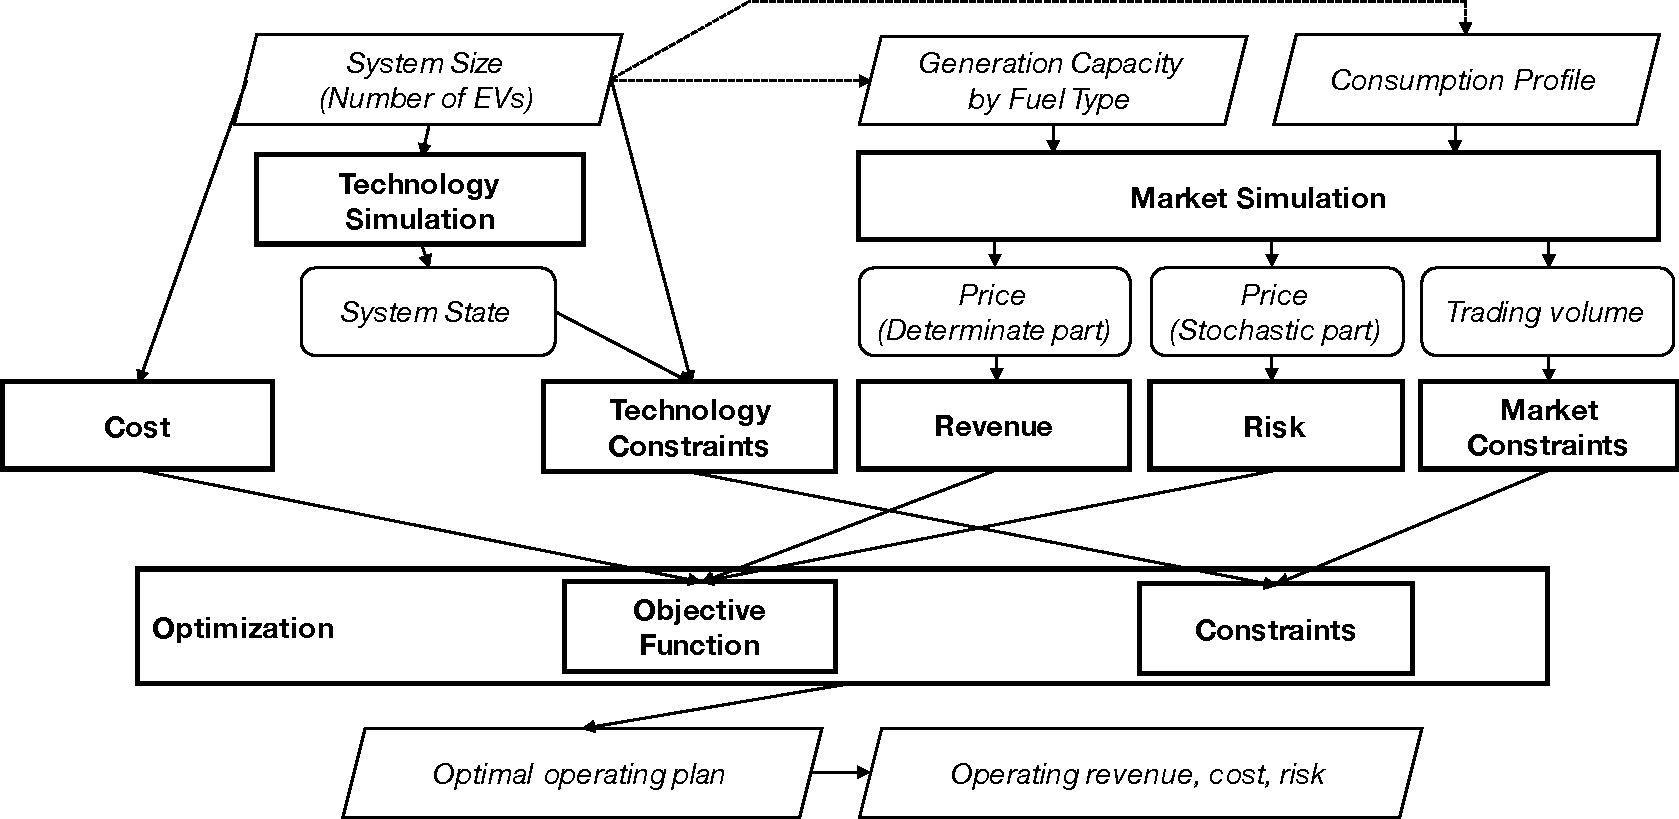
\includegraphics[scale=0.4]{Figures/ModelFlow.pdf}
	\caption{Flow chart of the techno-economic model}\
\end{figure}

Table \ref{tb:modules} offers an overview of all the modules and their inputs and outputs. The working flow of the model is illustrated by Figure \ref{fig:model-flow}.

With this model, we can evaluate the profitability and risk associated with a certain scale of flexibility management system in the power market and thus estimate the value of flexibility management market. Furthermore, we can assess the impact of driving factors including renewable penetration, cost reduction, and the possible diminishing return with increasing flexibility.

\section{Market-based modules}

\subsection{Revenue module}

In this study, we only consider explicit revenues from power markets. At each time step ($t$), the revenue ($\text{REV}_t$) is calculate as the amount of energy ($e_t$, in MWh) offered in each energy market segment ($i$), and/or amount of reserve ($r_t$, in MW) offered in each reserve market segment ($j$), multiplied by their corresponding prices ($\pi_t$, in \$/MWh or \$/MW). In reserve market, there are additional revenues from energy provision while the committed capacities are activated. The amount of energy delivered in reserve market is determined as a proportion of the committed reserve using a term of ratio ($\delta_t$, in MWh/MW). The total revenue within a given period of time ($T$) and a set of selected energy markets ($I$) and a set of  selected reserve markets ($J$), can be then computed as:

\begin{equation}
\label{eq:module-revenue}
\text{REV}=  \sum_{t}^{t \in T} \text{REV}_t = \sum_{t}^{t \in T} \left( \sum_{i}^{i \in I}  \pi_t^{e,i} (e_t^{d,i} - e_t^{c,i})  + \sum_{j}^{j \in J} (\pi_t^{e,j} \delta_t^{j} + \pi_t^{r,j}) r_t^j \right)
\end{equation}

where, $d$ and $c$ in the superscripts denote "discharge" (to release energy from flexibility resources to grids) and "charge" (to intake energy from girds to flexibility resources) respectively.  $e_t^{d,i}$, $e_t^{c,i}$, $r_t^{j}$, are endogenous variables of the whole model and decision variables of the optimization, which represent the operation plan of the flexibility resource in power markets.

$I$ and $J$ are determined according to the business case being studied. For example, we can set $I = \{Day~ahead\}$ and $J=\emptyset$ in order to the value of making arbitrage in day-ahead energy market. 

If there are multiple elements in $I \cup J$, it means the flexibility resource can be reallocated to make offers to different market segments, i.e. performing multitasking. These cases need to be carefully managed to comply with actual market rules. Detailed treatments regarding multitasking are illustrated in section \ref{sec:special}.

The ratios $\delta_t$ are computed based on the real control signal when data is available, or otherwise using system average ratios between total activated energy ($\hat{e}_t^{r,j}$) and the total reserve ($\hat{e}_t^{r,j}$) at each time step.

%\begin{equation*}
%\delta_t^j = \frac{\hat{e}_t^{r,j}}{\hat{r}_t^j}
%\end{equation*}

Price signals, $\pi_t^{e,i}$, $\pi_t^{r,j}$ and $\pi_t^{e,j}$, are inputs for the revenue module and may be retrieved either directly from historical data or from the outputs of market simulation module described in Section \ref{sec:market-simulation}.

We re-formulate Equation \eqref{eq:module-revenue} in form as:

\begin{equation*}
\text{REV} = \textit{\textbf{f}}~X
\end{equation*}

where $X$ is the vector for all desicion variables. For certain sets of market segments $I$ and $J$, $X$ can be derived using Equations \eqref{eq:decision-variable-1} - \eqref{eq:decision-variable-end} with $i \in I$ and $j \in J$.
\begin{equation}
\label{eq:decision-variable-1}
X =
\begin{bmatrix}
E^d \\ E^c \\ R
\end{bmatrix}
\end{equation}

\begin{equation}
E^d =
\begin{bmatrix}
E^{d,I(1)} \\ \vdots \\ E^{d,i} \\ \vdots \\ E^{d,I(|I|)}
\end{bmatrix} \\
E^{d,i} = 
\begin{bmatrix}
e_1^{d,i}\\e_2^{d,i}\\\vdots\\e_T^{d,i}
\end{bmatrix}
\end{equation}

\begin{equation}
E^c =
\begin{bmatrix}
E^{c,I(1)} \\ \vdots \\ E^{c,i} \\ \vdots\\ E^{c,I(|I|)}
\end{bmatrix} \\
E^{c,i} = 
\begin{bmatrix}
e_1^{c,i}\\e_2^{c,i}\\\vdots\\e_T^{c,i}
\end{bmatrix}
\end{equation}

\begin{equation}
\label{eq:decision-variable-end}
R =
\begin{bmatrix}
R^{J(1)} \\ \vdots \\R^{j} \\ \vdots \\ R^{J(|J|)}
\end{bmatrix} ~~~\\
R^{j} = 
\begin{bmatrix}
r_1^{j}\\r_2^{j}\\\vdots\\r_T^{j}
\end{bmatrix}
\end{equation}

Function $\textbf{f}$ can be obtained analogously using Eqution \eqref{eq:decision-f-revenue-1} $\sim$ \eqref{eq:decision-f-revenue-end} with $i \in I$ and $j \in J$.
\begin{equation}
\label{eq:decision-f-revenue-1}
\textit{\textbf{f}} =
\begin{bmatrix}
\Pi^{e,I}~|~&-\Pi^{e,I}~|~&\Pi^{e,J} \Delta^J + \Pi^{r,J}
\end{bmatrix}
\end{equation}

\begin{equation}
\Pi^{e, I} =
\begin{bmatrix}
\Pi^{e,I(1)}~|~&\dots~|~&\Pi^{e,I(|I|)}
\end{bmatrix} ~~~\\
\Pi^{e,i} = 
\begin{bmatrix}
\pi_1^{e,i}~\pi_2^{e,i}~\dots~\pi_T^{e,i}
\end{bmatrix}
\end{equation}

\begin{equation}
\Pi^{e,J} =
\begin{bmatrix}
\Pi^{e,J(1)}~|~&\dots~|~&\Pi^{e,J(|J|)}
\end{bmatrix} ~~~\\
\Pi^{e,j} = 
\begin{bmatrix}
\pi_1^{e,j}~\pi_2^{e,j}~\dots~\pi_T^{e,j}
\end{bmatrix}
\end{equation}

\begin{equation}
\Pi^{r,J} =
\begin{bmatrix}
\Pi^{r,J(1)}~|~&\dots~|~&\Pi^{r,J(|J|)}
\end{bmatrix} ~~~\\
\Pi^{r,j} = 
\begin{bmatrix}
\pi_1^{r,j}~\pi_2^{r,j}~\dots~\pi_T^{r,j}
\end{bmatrix}
\end{equation}

\begin{equation}
\label{eq:decision-f-revenue-end}
\Delta^J = diag (
\delta_1^{J(1)}, \dots , \delta_T^{J(1)}, \dots, \delta_1^{J(|J|)}, \dots, \delta_T^{J(|J|)})
\end{equation}

\subsection{Risk module}
In accordance with the revenue calculation, we consider the uncertain movement of price as the primary source of risk. Referring to similar works that performed risk management for flexibility sources, e.g. EV2G \cite{Alipour2017} and DER \cite{Han2017}, as well as for conventional energy trading companies \cite{Mohammadi-Ivatloo2013}, we developed a simple measure for risk control, by using the conditional value-at-risk (CVaR).

The CVaR (also named expected shortfall) as an extension of value-at-risk (VaR) can be defined as the difference between the expected profit and the average of potential profit values which are less than VaR \cite{Rockafellar2000}, shown as:

\begin{equation}
\label{eq:CVaR}
CVaR_\alpha (X) = \int_{\alpha}^{1} VaR_s(X) ds
\end{equation}

where $\alpha$ is the confidence level, and $X$ is the underlying (the price of energy/ reserve in our study). The VaR, as the negative of $\alpha$-quantile, can be computed as:

\begin{equation}
\label{VaR}
VaR_\alpha(X) = inf \{x \in \mathbb{R}~|~ P(X+x<0)\leq 1-\alpha\}
\end{equation}

Specially, in case the underlying variable subject to normal distribution, i.e. $X \sim \mathcal{N}(\mu,\,\sigma^{2})\,$, we can derive the CVaR as:

\begin{equation}
CVaR_\alpha(X) = \mu - \sigma \frac{\phi(\Phi^{-1}(\alpha))}{1-\alpha}
\end{equation}
%http://blog.smaga.ch/expected-shortfall-closed-form-for-normal-distribution/
where, $\Phi(\cdot)$ is cumulative distribution function and $\phi(\cdot)$ is the probability density function of normal distribution.

Alternatively, if the uncertainties are dealt with in a discrete manner, the CVaR can be calculated as\cite{Rockafellar2000}:

\begin{equation}
CVaR_\alpha (X) = \underset{\zeta}{max}\left( \zeta - \frac{1}{1-\alpha} \sum_{s} P(X,s) (\zeta - f(X,s))\right)
\end{equation}
where, $P(X,s)$ is the probability distribution function of $X$ in the scenario $s$ and $f(X,s)$ is the profit function in the scenario $s$. $\zeta$ is an auxiliary variable constrained by

\begin{equation*}
\zeta - f(X,s) \leq \zeta_s
\end{equation*}
\begin{equation*}
\zeta_s \geq 0
\end{equation*}

In our study, price terms $\tilde{\pi}$ are assumed to comprise a determinate part $\pi$ and an independent stochastic deviation $\epsilon$:
\begin{equation}
\label{eq:price-error}
\tilde{\pi_t}= \pi_t + \epsilon_t
\end{equation}

Since the stochastic terms $\epsilon$ are assumed to be uncorrelated to each other, the CVaR of our portfolio that is built by  $X^T = [E^d~|~E^c~|~R]$
in Equation \eqref{eq:decision-variable-1} can be aggregated as:

\begin{equation}
\begin{aligned}
CVaR =\sum_{t}^{t \in T} \{&\\
&\sum_{i}^{i \in I}  CVaR(\tilde{\pi_t}^{e,i}) (e_t^{d,i} - e_t^{c,i})  \\
&+ \sum_{j}^{j \in J} \left(CVaR(\tilde{\pi_t}^{e,j}) \delta_t^{j} + CVaR(\tilde{\pi_t}^{r,j})\right) r_t^j \\
&\}
\end{aligned}
\end{equation}

Analogous to the formation in preceding section, the risk module is also formulated in vector and matrix form.

\begin{equation*}
CVaR= \textit{\textbf{f}}
\begin{bmatrix}
E^d \\ E^c \\ R
\end{bmatrix}
\end{equation*}

where \textit{\textbf{f}} is calculated as:

\begin{equation}
\textit{\textbf{f}} =
\begin{bmatrix}
CVaR(\Pi^{e,I})\\-CVaR(\Pi^{e,I})\\CVaR(\Pi^{e,J}) \Delta^J + CVaR(\Pi^{r,J})
\end{bmatrix}^T
\end{equation}

\subsection{Market simulation module}
\label{sec:market-simulation}
As has been illustrated in the literature review (Chapter \ref{ch:LitRev}), valuation of flexibility with a dynamic market condition is still a challenging task. While investment decisions are extensively concerned with long-term trends, profitability of arbitrage sensitively depends on short-term price movement in high resolution. This is distinguishing from conventional electricity generators for whom a long-term forecast with coarse resolution is sufficient, and visual arbitrageurs who have almost no investments on infrastructures and may perform decision-makings with a short-term perspective. A holistic approach combining these researches were taken sometimes \cite{Rastler2010}\cite{Eyer2010} but may easily bring in unnecessary complexity and lead to an overwhelming demand of resources, which are not essential for our study.

Therefore, in this thesis, we customized a market model based on existing researches by re-focusing on factors that are most relevant to our research questions, and simplifying many other aspects of the power system and markets. Our market model is generally a statistic model built on observations of historical data, but a physical sub-model is incorporated as well to study the impacts of some relevant variables whose features are not well captured by empirical observations.

The approach for market simulation differentiates between energy markets and reserve markets. 

The energy markets are usually matured and with abundant degree of competition, so that we can employ an idealistic market model where the price formation is governed by the short run marginal costs (SRMCs) \cite{Grunewald2012} \cite{Grunewald2012a}. This allows us to leverage a merit-order model to simulate the price levels, which are widely adopted as is summarized in Chapter \ref{ch:LitRev}. 

The design of reserve markets, on the contrary, is not as straightforward as energy markets, which pose challenges for robust modeling. Besides, the market mechanisms vary spatially and temporally as is analyzed previously. Therefore, we adopt a pure statistic model for reserve market without involving any physical modeling.

\subsubsection{Day-ahead energy market}

The simulation for day-ahead energy market is preliminarily based on work done by \cite{Grunewald2012a} where the merit-order curve at supply shortage and surplus is modeled by an uplift effect. We further extend this work to capture the limits of flexibility provision in current energy markets so that we can simulate the market conditions when the flexibility become a challenge with growing renewables and/ or the flexibility becomes ubiquitous.

In \cite{Grunewald2012a}, the peak price during periods of high demand is explained as fewer participants remain with spare generating capacity, putting these actors in a stronger bidding position to mark up the price. In contrast, when demand is low and plants with high SRMCs would not operate so further reduction in generation would favor plants with low SRMCs and thus reverse the bidding position. In both cases, the less available capacity remains, the stronger bidding position for the remaining players, which happens at the two end of merit-order curve where the prices are driven up or down to significantly depart from the marginal cost. The symmetric effect is model with a uplift function:

\begin{equation}
U_t^g = 1 + \kappa~e^{-\alpha\left(\frac{C_t^g -P^g_t }{C^g}\right)}
\end{equation}

where $g$ denote the class of generation in merit order, e.g. peak, flexible, inflexible, etc. ($\kappa$) and ($\alpha$) are the parameters which can be obtained empirically \cite{Cox2009}. In case of peak period, $C^g_t$ represents total avaiable generation capacity of class $g$ and $P^g_t$ is the output of genertion of class g. During period of generation surplus, $C^g_t$ is the remaining generation capacity while $P^g_t$ is the curtailment required.

The middle of merit order curve can be modeled with a linear relationship.

Since the SRMCs of renewable generations are almost zero or even negative when they are remunerated by renewable support schemes, their position in power market is distinguishing from other generation players. Therefore, we employed the residual load, i.e. the load net of renewable generation, which has been introduced previously. We denote the residual load as $L^{res.}$ here.

According to the discussion above, the uplifts will occur when $L^{res.}$ exceeds the capacity of mid-merit generations and when $L^{res.}$ is smaller than operating capacity of inflexible generations.

Therefore, the merit order model for price formation can be formulated as:

\begin{equation}
\label{eq:merit-order-model}
\pi_t = \begin{cases}
\dot{\pi}_t \left[1 + \kappa~e^{-\alpha\left(\frac{C_t^g -P^g_t }{C^g}\right)} \right] & L^{res.}_t \leq C^{inflex.}_t\\ 
\dot{\pi}_t ~\kappa~\frac{P^g_t}{C_t^g} & C^{inflex.}_t < L^{res.}_t < C^{inflex.}_t+ C^{mid.}_t\\
\dot{\pi}_t  \left[1 + \kappa~e^{-\alpha\left(\frac{C_t^g -P^g_t }{C^g}\right)} \right] & L^{res.}_t \geq C^{inflex.}_t + C^{mid.}_t\\
\end{cases}
\end{equation}

In order to derive the value of generation capacity of each class, an investigation into the flexibility of power plants is necessary.

\begin{figure}[h!]
	\label{fig:power-plant-flexibility}
	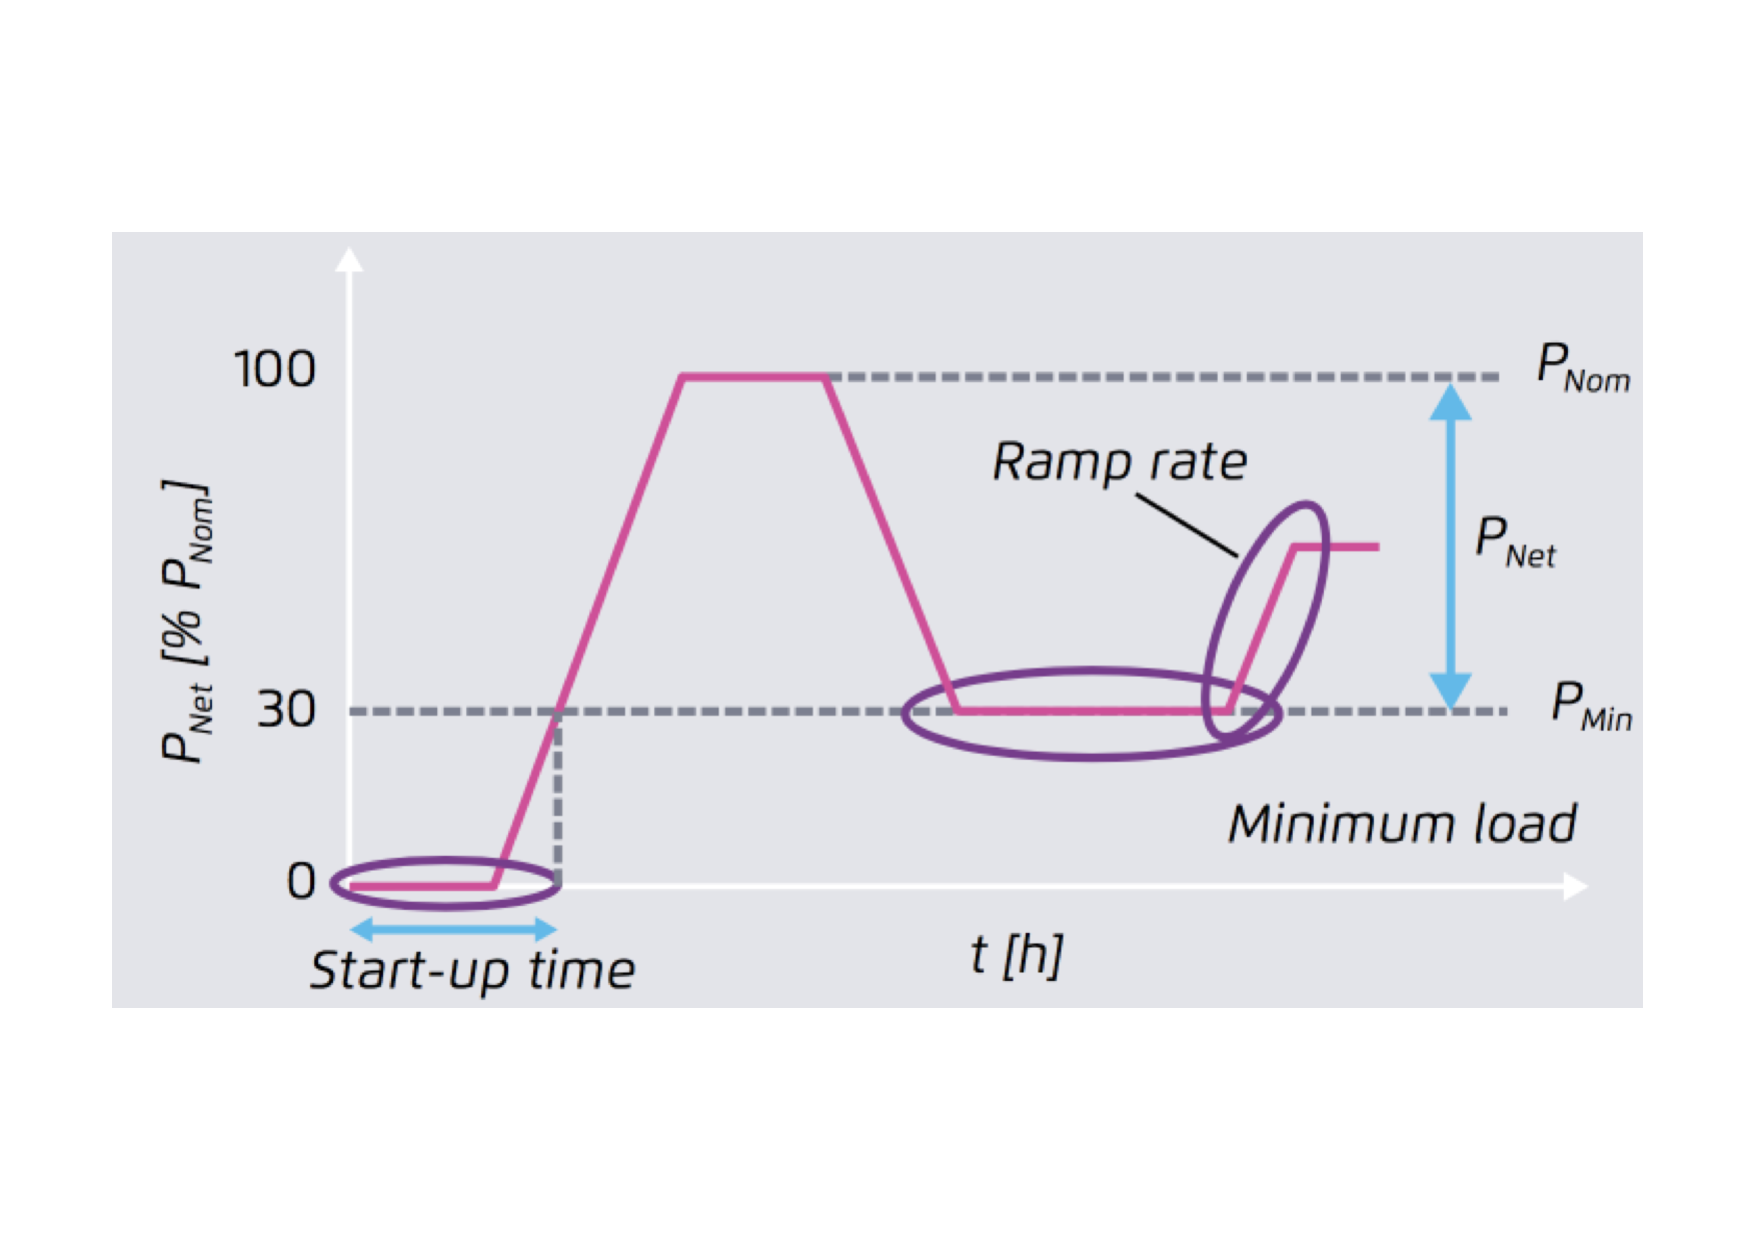
\includegraphics[scale=0.4]{Figures/PowerPlantFlexibility.pdf}
	\caption{Qualitative representation of key flexibility parameters of a power plant\cite{AgoraEnergiewende2017}}\
\end{figure}

The flexibility of a power plant can be characterized by three key features\cite{AgoraEnergiewende2017} (Figure \ref{fig:power-plant-flexibility}): 
\begin{itemize}
	\item Overall bandwidth of operation: the range of output between minimum and maximum load;
	\item Ramp rate: the speed of adjusting output;
	\item Start-up time: the time required to attain stable operation from standstill
\end{itemize}

%https://www.researchgate.net/profile/Alejandro_Hoese
If a power plant can adjust its load from zero to nominate capacity within a time block in the day-ahead market (typically 1 hour), it can be deemed with infinite flexibility in the day-ahead market. This applies to most type generations including solar, wind, hydro and electrochemical systems, etc., except for generations using steam turbines \cite{AgoraEnergiewende2017}, including nuclear, coal-, oil and gas-steam, etc. The gas turbines can be ramped up to full capacity within typically 30 minutes\cite{Siemens}\cite{GE} so can be considered as flexible generation.

For a steam-turbine power plant, the minimum operational load is about 25-60\% of its nominal capacity while the time required to start from standstill is longer than 2 hours \cite{AgoraEnergiewende2017}. Therefore, they are treated as limited flexible sources.

For limited flexible generations, an empirical analysis is performed to determine its bounded flexibility. The procedure for a certain generation source is decribed as following and shown as Figure \ref{fig:bounded-flexibility}:

\begin{figure}[h!]
	\label{fig:bounded-flexibility}
	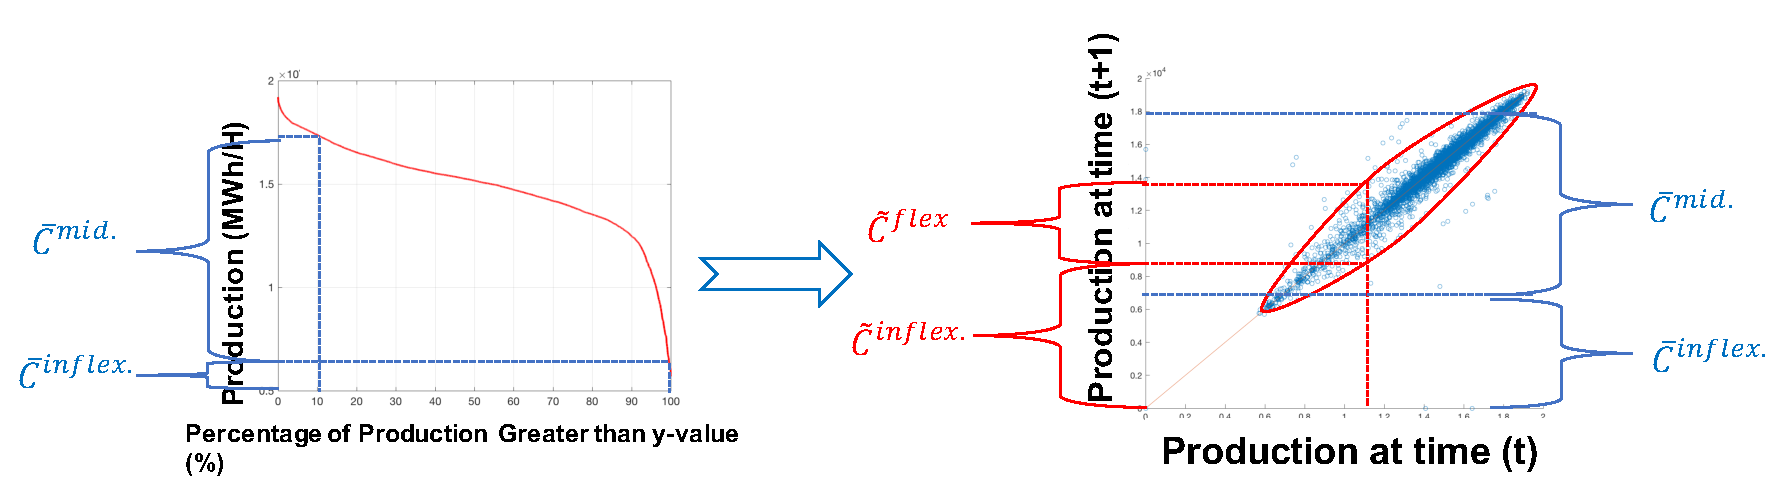
\includegraphics[scale=0.4]{Figures/BoundedFlexibility.pdf}
	\caption{Schematic illustration of determining bounded flexibility for limited flexible generations}\
\end{figure}


\begin{enumerate}
	\item Make the duration curve of the generation data, and obtain $\overline{c}^{mid.}$ which is the range that the generation source is operating for over 10-99\% of the overall period and $\overline{c}^{inflex.}$ which is the range that the generation is operating of more than 99\% of the time.
	\item Determine the envelop lines which limit the production at time $t+1$ based on production at time $t$. With a certain production $p_{t}$, $p_{t+1}$ is bounded within $\tilde{c}^{flex}$, and there is a range of production $\tilde{c}^{inflex}$ that is not economically viable to be curtailed.
	\item Finally, we find the relationship that map the production at time $t$ to flexible capacity at time $t+1$ as: 
	\begin{equation}
	\begin{aligned}
	c^{inflex.}_{t+1} &= \mathcal{C}^{inflex}(p_t)\\ &=max\{\tilde{c}^{inflex.}_t,~\overline{c}^{inflex.}\}
	\end{aligned}
	\end{equation}
	\begin{equation}
	\begin{aligned}
	c^{flex.}_{t+1} &= \mathcal{C}^{flex.}(P_t) \\ & =min\{\tilde{c}^{flex.}_t+\tilde{c}^{inflex.}_t,~\overline{c}^{mid.}+\overline{c}^{flex}_t \} - \tilde{c}^{inflex.}_t
	\end{aligned}
	\end{equation}
	\begin{equation}
	\begin{aligned}
	c^{peak}_{t+1} &= \mathcal{C}^{peak}(P_t) \\ & =max\{\tilde{c}^{flex.}_t+\tilde{c}^{inflex.}_t -(\overline{c}^{mid.}+\overline{c}^{flex}_t),0 \}
	\end{aligned}
	\end{equation}
\end{enumerate}

When the load exceeds the flexible range of these sources, they are no long able to participate in the bidding so these portion of capacity shall be deducted from the overall capacity for the calculation using Equation \eqref{eq:merit-order-model}.

Finally, a regression is performed to determine the parameters in Equation \eqref{eq:merit-order-model} using empirical observations. The errors between a regressed value $\pi_t$ and an actual value $\tilde{\pi}_t$ would be analyzed as the uncertainty of price movement and used for risk controlling as is discussed in risk module. 

With a established merit-order model for day-ahead energy market, we can re-simulate the price with changed market condition, e.g. altered generation capacity mix.

\subsubsection{Real-time energy market and reserve market}

In electricity markets, large portion of energy is usually traded in day-ahead market \cite{Kardakos2013}. There are significate dependences of the real-time (intraday, balancing) energy price on day-ahead price \cite{Woo2016}. Therefore, for real-time energy prices, we adopt a simplex empirical analysis based on comparing the results from day-ahead price simulation and actual market data:

\begin{equation}
\pi^{RT}_t = \kappa (\pi^{DA}_t + \alpha) + \epsilon_t
\end{equation}
where, $\kappa$ and $\alpha$ are terms to adjust the determinate bias between day-ahead and real-time price, while $\epsilon_t$ represents the stochastic movement of real-time price. 

For reserve market, only an empirical model is used as is discussed previously.

\subsection{Market constraints}

The market constraints are a list of limits to make sure that the operation of flexibility resource (determined by $X$ in Equation \eqref{eq:decision-variable-1}) would not violate the actual market rules and market conditions.

Generally, these constraints can be formulated as

\begin{equation}
\begin{bmatrix}
\Gamma^d~~|& \Gamma^c~~|&\Gamma^r
\end{bmatrix}
X \leq \textit{\textbf{b}}
\end{equation}

Most of the market constraints are derived from the market rules so will be introduced in case studies where specific markets are being studies. 

%Capacity constraints:
%\begin{equation}
%r_t^j \leq \hat{r}_t^j ~~~ j \in J
%\end{equation}

%Since in this study high penetration of flexibility resources will be investigated, 

%Day-ahead
%\begin{equation}
%\hat{e}_t^i - \hat{e}_t^{peak} \leq e_t^{d,i} - e_t^{c,i} \leq \hat{e}_t^i - \hat{e}_t^{base} ~~~ i \in \{Day~Ahead\}
%\end{equation}

%Real-time
%PJM revised order +/- 10% of the DA offer
%Germany volume limited





\section{Technology-based modules}

\subsection{Cost module}
\label{sec:cost}
In this thesis, we categorize all costs into two groups: operation-independent and operation-dependent costs.

\subsubsection{Operation-independent costs}
The first group mainly including the initial capital outlay for purchasing the devices and systems, plus the fixed operating and maintenance (O\&M) costs which include miscellaneous items such as the insurance, employee salaries, etc. 

The initial capital cost for a storage system can be divided into two components: an energy-based component, approximately linear to the energy capacity of the system (denoted $\overline{s}$, in MWh), and a power-based component, approximately linear to the power rate of the system (denoted $\overline{r}$, in MW) \cite{Megel2017}. Additionally, we add a component representing the size-invariant costs such as the cost for software. Thereby, the initial capital cost can be computed as:

\begin{equation}
C^{ini} = C^s \overline{s} + C^r \overline{r} + C^0
\end{equation}

where, the coefficients can be obtained empirically either by screening actual market data or from literature. In addition, since the system cost for battery storage is falling rapidly, a learning rate of \textit{ca.} 14\% per annum can be taken to build future scenarios\cite{Nykvist2015}.

The initial capital cost is then annualized by using the concept of equivalent annual cost (EAC):

\begin{equation}
C^{EAC} = \frac{C^{ini}}{\frac{1 - \frac{1}{(1+r)^a}}{r}}
\end{equation}

where $r$ is the discount rate and $a$ is the lifespan of the system in number of years.

The discount rate can be established from the Weighted Average Cost of Capital (WACC) which depends on the financial conditions of different players. A typical WACC in the United States is \textit{ca.} 4-6\% for a municipal utility, 7-8\% for a regulated utility and over 10\% for independent power producer\cite{Rastler2010}. In this study, a discount rate of 10\% is taken unless otherwise stated.

For fixed O\&M costs, $C^{fO\&M}$ which is difficult to calculate precisely, an assumption of 2\% of the initial capital cost is taken, referring to \cite{Rastler2010}. The fixed O\&M costs are added directly to the annualized capital cost to get the total fix costs (in \$/year):

\begin{equation}
C^{fix} = C^{EAC} +  C^{fO\&M}
\end{equation}

The annualized fix cost will finally be compared with the operating revenue calculated from other module to assess the profitability.

\subsubsection{Operation-dependent costs}

Operation-dependent costs primarily refer to the degradation costs, which is specially an issue for battery-based energy storage systems\cite{Barre2013}.

However, as has been reviewed and analyzed in \cite{Megel2017}, there exists no single degradation model that is widely accepted among the literature and applicable for all cases, due to the complexity of this problem. The reasons can be summarized as following:
\begin{itemize}
	\item Modelling battery degradation itself is a complex engineering problem as it is affected by a list of physical parameters, including the degree-of-discharge (DoD), state-of-charge (SoC), charging/discharging rate, temperature, etc.\cite{Barre2013}
	\item The choice of degradation model affects the convex relaxation when degradation effects are included in an optimization problem, the model selection is driven by the requirements of mathematical realization. \cite{Megel2017}
\end{itemize}

Degradation costs can be neglected while operating life time is longer than designed life time, which is generally valid for non-battery energy systems \cite{Bradbury2014}\cite{Zafirakis2016}\cite{Connolly2011}. Some research works studying battery system also made the same assumption  \cite{Byrne2012}\cite{McConnell2015}\cite{Sioshansi2009}. The breakeven point of operational frequency where the degradation of battery storage system can be ignored was concluded to be less than 0.5-1.5 full-cycle equivalent energy throughput per day\cite{Megel2017}. Nonetheless, it was also pointed out by \cite{Megel2017} that while assuming degradation cost being zero, the operational planner would tend to operate the system more frequently, which would possibly in turn to violate the assumption of zero-degradation.

Such a combined investment and operation problem is hard to be incorporated in an optimization, so in our study we first use a simple degradation cost model where the cost is linear to the \textit{energy throughput} $|e^t|$ as a damping term in the optimization and examine it \textit{ex-post}, i.e. if the actual operating life is not reached the degradation cost will be exempted from the final profit calculation. A linear relationship between the degradation and $|e^t|$ is a common technique used in researches for estimating battery degradation\cite{Byrne2012}\cite{Berrada2016}.

Denoting the damping factor for degradation as $\zeta$, we can formulate the degradation damping as:

% THIS IS WRONG
\begin{equation}
\label{eq:degradation-damping}
C^{degradation}_t = \zeta (\sum_{i}^{i \in I}(e_t^{d,i}+e_t^{c,i})+\sum_{j}^{j \in J}(\delta_t^{j,+}+\delta_t^{j,-})r_t^j)
\end{equation}

where, the energy to reserve ratios are separated to positive and negative components:
\begin{equation}
\label{eq:ratio-pos}
\delta_t^{j,+} = \begin{cases}
\delta_t^j & \delta_t^j  \geq 0\\
0 & \delta_t^j  < 0
\end{cases}
\end{equation}
\begin{equation}
\label{eq:ratio-neg}
\delta_t^{j,-} = \begin{cases}
0 & \delta_t^j  \geq 0\\
-\delta_t^j & \delta_t^j  < 0
\end{cases}
\end{equation}

It can be noticed that when a virtual arbitrage is conducted where some $e_t^{d,i}$ and $e_t^{c,i}$ are offset, it will activate the degradation damping with Equation \eqref{eq:degradation-damping} while there are no real physical processes causing degradation. This will be corrected in final profit calculation but in decision making process using optimizations we keep it as it is intended to restrict the virtual arbitrage.

Similar to Equation \eqref{eq:decision-f-revenue-end}, we reconstruct the diagonal matrices with the decomposed ratios from Equation \eqref{eq:ratio-pos} and \eqref{eq:ratio-neg}.
\begin{equation}
\Delta^+ = diag (
\delta_1^{J(1),+}, \dots , \delta_T^{J(1),+}, \dots, \delta_1^{J(|J|),+}, \dots, \delta_T^{J(|J|),+})
\end{equation}
\begin{equation}
\Delta^- = diag (
\delta_1^{J(1),-}, \dots , \delta_T^{J(1),-}, \dots, \delta_1^{J(|J|),-}, \dots, \delta_T^{J(|J|),-})
\end{equation}

The matrix of coefficient for degradation is the derived complying with the form of market modules:

\begin{equation*}
Cost^{degradation} = \begin{bmatrix}
Z^{I}~|~&Z^{I}~|~& \zeta (\Delta^{+} +\Delta^{-})
\end{bmatrix} \begin{bmatrix}
E^d \\ E^c \\ R
\end{bmatrix}
\end{equation*}

where,
\begin{equation*}
Z^I = \begin{bmatrix}
Z^{I(1)}~~|&\dots~~|&Z^i~~|&\dots~~|&Z^{I(|I|)}
\end{bmatrix}~~~
Z^i = \zeta \cdot I_{T\times T} ~~~ \forall i \in I
\end{equation*}

$I_{T \times T}$ is a ($T \times T$) identity matrix. 

\subsection{Technology simulation module}
The technology simulation is applied to determine the state of the system, which would be used primarily for calibration of technology constraints but also for \textit{ex-post} analysis.

\subsubsection{Energy Storage}
Regardless of the type of technology, an energy storage system consists of three functional units, i.e. power input, power output, and storage. Each function unit is associated with an efficiency, i.e. conversion efficiencies of charging, discharging and storage efficiency, denoted as $\eta_c$, $\eta_d$ and $\eta_s$ respectively.

Since the ramp up time for a typical storage system is neglectable comparing to the time resolution in our study, the state of power input and output are deemed as strictly following the operational plan without transient process.

For the state of storage, we define a term, $s$ (in MWh), which is the energy stored in the device, i.e. the State-of-Charge (SoC) multiplied by its maximum energy capacity. The state is determined using Equation \ref{eq:tech-ESS}.

\begin{equation}
\label{eq:tech-ESS}
s_t = \eta_s s_{t-1} + \eta_c (\sum_{i}^{i \in I} e_t^{c,i} + \sum_{j}^{j \in J}\delta_t^{j,-}r_t^j)- \frac{1}{\eta_d} (\sum_{i}^{i \in I} e_t^{d,i} + \sum_{j}^{j \in J}\delta_t^{j,+}r_t^j)
\end{equation} 

In order to formulate Equation \eqref{eq:tech-ESS} in matrix form, we first introduce a matrix denoted $H$:
\[
H
=
\begin{bmatrix}
\eta_s^0 & 0 & 0 &  \dots & 0 \\
\eta_s^1 & \eta_s^0 & 0 &  \dots & 0 \\
\eta_s^2 & \eta_s^1 & \eta_s^0 &  \dots & 0 \\
\vdots & \vdots & \vdots &  \ddots & \vdots \\
\eta_s^{T-1} & \eta_s^{T-2} & \eta_s^{T-3} & \dots & \eta_s^0 \\
\end{bmatrix}
\]
\newline
Then $M$ is used to construct $H^I$ and $H^J$ with a given pair of sets of market segments $I$ and $J$.
\begin{equation*}
H^I = \begin{bmatrix}
H^{I(1)}~~|&\dots~~|&H^i~~|&\dots~~|&H^{I(|I|)}
\end{bmatrix}~~~
H^i = H ~~~ \forall i \in I
\end{equation*}
\begin{equation*}
H^J = \begin{bmatrix}
H^{J(1)}~~|&\dots~~|&H^j~~|&\dots~~|&H^{J(|J|)}
\end{bmatrix}~~~
H^j = H ~~~ \forall j \in J
\end{equation*}
Finally, we can derive the matrix form of Equation \eqref{eq:tech-ESS}.
\begin{equation}
\label{eq:tech-ESS-M}
S = \eta_s H S_0 + \begin{bmatrix}
-\frac{1}{\eta_d} H^I~~|& \eta_c H^I~~|& H^J (-\frac{1}{\eta_d} \Delta^{+} + \eta_c \Delta^{-})
\end{bmatrix} X
\end{equation}
where, $S$ and $S_0$ are vectors for the temporal and initial state, respectively.
\begin{equation*}
S = \begin{bmatrix}
s_1~~s_2~~\dots~~s_T
\end{bmatrix}^T
\end{equation*}
\begin{equation*}
S_0 = \begin{bmatrix}
s_0~~s_0~~\dots~~s_0
\end{bmatrix}^T
\end{equation*}

In order to make it more compact, we reformulate Equation \eqref{eq:tech-ESS-M} as:

\begin{equation}
\label{eq:state-ESS-M-1}
S = \textit{\textbf{h}}_0 + \textit{\textbf{h}}~X
\end{equation}
where
\begin{equation}
\label{eq:state-ESS-M-2}
\textit{\textbf{h}}_0 =  \eta_s H S_0
\end{equation}
\begin{equation}
\label{eq:state-ESS-M-3}
\textit{\textbf{h}} = \begin{bmatrix}
-\frac{1}{\eta_d} H^I~~|& \eta_c H^I~~|& H^J (-\frac{1}{\eta_d} \Delta^{+} + \eta_c \Delta^{-})
\end{bmatrix}
\end{equation}
\subsubsection{Electric Vehicle}

%Charging rate: https://www.tesla.com/support/home-charging-installation
Electric vehicle to grid systems are fundamentally battery energy storage systems in term of their physical dynamics. Therefore, they can be modeled generally using the same approach as in preceding paragraphs. However, there are several attributes that uniquely characterize electric vehicle to grid systems compared to normal battery storages:

\begin{itemize}
	\item The availability of an EV2G system, in terms of delivering both energy (in MWh) and capacity reserve (in MW), is dynamic rather than static, since the number of EVs connected in the power grid is changing all the time with the behaviors of plug-in/ plug-out.
	\item The energy stored in the system will be consumed not only for delivering our targeted services (arbitrage or balancing), but also for driving of EVs themselves. This part of costs will be implicitly captured by the revenue module using Equation \eqref{eq:module-revenue}, which will distort the real value of services provided for the grid. 
\end{itemize}

Therefore, two main modifications are made to adapt the model of ESSs for better representing the EV2G systems: 

\begin{enumerate}
	\item The EV2G system is modeled as a dynamic ESS by taking into consideration the connection/ disconnection of EVs to/ from the grids.
	\item The costs of energy consumed for driving are accounted, following the original plan, i.e. without controlling algorithm for grid services, and added back to the revenue in Equation \eqref{eq:module-revenue}.
\end{enumerate}

In order to implement the first measure, we introduce additional terms to represent the number of EVs entering ($n_t^+$), leaving ($n_t^-$) and remain in ($n_t$) the system at each time step. 
\begin{equation}
\label{eq:EV-number}
n_t = n_{t-1} + n_t^+ - n_t^-
\end{equation}

Thereby the state equation for an EV2G system is written as:
\begin{equation}
\label{eq:tech-EV}
\begin{aligned}
s_t = & \eta_s s_{t-1} + \eta_c (\sum_{i}^{i \in I} e_t^{c,i} + \sum_{j}^{j \in J}\delta_t^{j,-}r_t^j)- \frac{1}{\eta_d} (\sum_{i}^{i \in I} e_t^{d,i} + \sum_{j}^{j \in J}\delta_t^{j,+}r_t^j) \\
&+ s_t^+ n_t^+ - s_t^- n_t^-
\end{aligned}
\end{equation} 
\newline
The matrix form of Equation \eqref{eq:EV-number} is as following:
\begin{equation}
\label{eq:EV-number-M}
N = I_{T \times T} N_0 + L_{T \times T} N^+ -L_{T \times T} N^- 
\end{equation}
where, $L_{T \times T}$ is a ($T \times T$) identity lower triangular matrix. The rest matrices are defined as following
\begin{equation*}
N = \begin{bmatrix}
n_1~~n_2~~\dots~~n_T
\end{bmatrix}^T
\end{equation*}
\begin{equation*}
N_0 = \begin{bmatrix}
n_0~~n_0~~\dots~~n_0
\end{bmatrix}^T
\end{equation*}
\begin{equation*}
N^+ = \begin{bmatrix}
n_1^+~~n_2^+~~\dots~~n_T^+
\end{bmatrix}^T
\end{equation*}
\begin{equation*}
N^- = \begin{bmatrix}
n_1^-~~n_2^-~~\dots~~n_T^-
\end{bmatrix}^T
\end{equation*}
\begin{equation*}
S^+ = diag(s_1^+, s_2^+, \dots, s_T^+
)
\end{equation*}
\begin{equation*}
S^- = diag(s_1^-, s_2^-, \dots, s_T^-)
\end{equation*}
\newline
Analogously, translating Equation \eqref{eq:tech-EV} to matrix form leads to:

\begin{equation}
\begin{aligned}
S = &~ \eta_s H S_0 + H S^+ N^+ - H S^- N^- \\
&~+ \begin{bmatrix}
-\frac{1}{\eta_d} H^I~~|& \eta_c H^I~~|& H^J (-\frac{1}{\eta_d} \Delta^{+} + \eta_c \Delta^{-})
\end{bmatrix} X
\end{aligned}
\end{equation}
which can be reformulated as:
\begin{equation}
\label{eq:state-EV-M-1}
S = \textit{\textbf{h}}_0 + \textit{\textbf{h}}~X
\end{equation}
where
\begin{equation}
\label{eq:state-EV-M-2}
\textit{\textbf{h}}_0 =  \eta_s H S_0 + s^+ H N^+ - s^- H N^-
\end{equation}
\begin{equation}
\label{eq:state-EV-M-3}
\textit{\textbf{h}} = \begin{bmatrix}
-\frac{1}{\eta_d} H^I~~|& \eta_c H^I~~|& H^J (-\frac{1}{\eta_d} \Delta^{+} + \eta_c \Delta^{-})
\end{bmatrix}
\end{equation}

\subsection{Technology constraints}
\label{sec:tech-constraints}
The technology constraints are set to ensure the operation plan is fulfilled physically by the system.

\subsubsection{Energy storage}
Firstly, the charging/ discharging rate shall be bounded at its maximum rate ($\overline{r}$, assuming symmetric for charge and discharging).

\begin{equation}
0 \leq \frac{1}{\Delta t}\sum_{i}^{i \in I} e^{d,i}_t + \sum_{j}^{j \in J} r_t^j \leq \overline{r}~~~ \forall t \in T
\end{equation}

\begin{equation}
0 \leq \frac{1}{\Delta t}\sum_{i}^{i \in I} e^{c,i}_t + \sum_{j}^{j \in J} r_t^j \leq \overline{r}~~~ \forall t \in T
\end{equation}

It can be noticed that opposite movement of charging/ discharging in different markets are not offset in the constraints. This implies virtual arbitrageurs are not allowed to make deals that cannot be afforded physically although the physical systems are not actually activated.

Meanwhile, the energy stored is restricted as well.

\begin{equation}
0 \leq s_t \leq \overline{s}~~~ \forall t \in T
\end{equation}

Replacing $s_t$ using Equation \eqref{eq:tech-ESS}, the contraint is formulated as:
\begin{equation}
0 \leq \eta_s s_{t-1} + \eta_c (\sum_{i}^{i \in I} e_t^{c,i} + \sum_{j}^{j \in J}\delta_t^{j,-}r_t^j)- \frac{1}{\eta_d} (\sum_{i}^{i \in I} e_t^{d,i} + \sum_{j}^{j \in J}\delta_t^{j,+}r_t^j) \leq \overline{s}
\end{equation}

Applying the matrix format of the equations, we can get the constraints re-formulated the constraints of rates as:

\begin{equation}
- \frac{1}{\Delta t} \begin{bmatrix}
\overbrace{ I_{T\times T}|\dots|I_{T\times T}}^\text{|I|}|\overbrace{O_{T\times T}|\dots|O_{T\times T}}^\text{|I|}|\overbrace{ I_{T\times T}|\dots|I_{T\times T}}^\text{|J|}| 
\end{bmatrix} X \leq 0
\end{equation}

\begin{equation}
- \frac{1}{\Delta t} \begin{bmatrix}
\overbrace{ O_{T\times T}|\dots|O_{T\times T}}^\text{|I|}|\overbrace{I_{T\times T}|\dots|I_{T\times T}}^\text{|I|}|\overbrace{ I_{T\times T}|\dots|I_{T\times T}}^\text{|J|}| 
\end{bmatrix} X \leq 0
\end{equation}

\begin{equation}
\label{constraint:ESS-capacity}
\frac{1}{\Delta t} \begin{bmatrix}
\overbrace{ I_{T\times T}|\dots|I_{T\times T}}^\text{|I|}|\overbrace{O_{T\times T}|\dots|O_{T\times T}}^\text{|I|}|\overbrace{ I_{T\times T}|\dots|I_{T\times T}}^\text{|J|}| 
\end{bmatrix}X \leq \overline{R}
\end{equation}
\begin{equation}
\label{constraint:ESS-capacity-2}
\frac{1}{\Delta t} \begin{bmatrix}
\overbrace{ O_{T\times T}|\dots|O_{T\times T}}^\text{|I|}|\overbrace{I_{T\times T}|\dots|I_{T\times T}}^\text{|I|}|\overbrace{ I_{T\times T}|\dots|I_{T\times T}}^\text{|J|}| 
\end{bmatrix}X \leq \overline{R}
\end{equation}

where $O_{T \times T}$ is a $T \times T$ zero matrix and
\begin{equation*}
\overline{R} = \begin{bmatrix}
\overbrace{\overline{r}, \dots, \overline{r}}^\text{T}
\end{bmatrix}^T
\end{equation*}


The constraints of storage are formulated as:
\begin{equation}
\label{constraint:ESS-energy-1}
-\textit{\textbf{h}}~X \leq \textit{\textbf{h}}_0
\end{equation}
\begin{equation}
\label{constraint:ESS-energy-2}
\textit{\textbf{h}}~X \leq \overline{S} -  \textit{\textbf{h}}_0
\end{equation}
where, $\textit{\textbf{h}}$ and $\textit{\textbf{h}}_0$ are determined by Equation \eqref{eq:state-ESS-M-1} to \eqref{eq:state-ESS-M-3}, and
\begin{equation*}
\overline{S} = \begin{bmatrix}
\overbrace{\overline{s}, \dots, \overline{s}}^\text{T}
\end{bmatrix}^T
\end{equation*}

\subsubsection{Electric vehicle to grid}

The constraints for ESS are generally portable for the EV2G systems, by simplying re-using Equation \eqref{eq:state-EV-M-1} to \eqref{eq:state-EV-M-3} to derive $\textit{\textbf{h}}$ and $\textit{\textbf{h}}_0$, and replacing the upper bound limit in Equation \ref{constraint:ESS-capacity} with

\begin{equation}
\overline{R} = \overline{r}N
\end{equation}
where, $N$ is determined by Equation \eqref{eq:EV-number-M}. 




\section{Optimization Engine}
The performance of a flexibility resource depends primarily on the operation plan, which is represented as $X$ (Equation \ref{eq:decision-variable-1}). In order to value the market of technology vendors supplying flexibility to actors in power markets, we need to find reasonable operation patterns that simulate the behaviors of those players. For this sake, we employ an optimization engine. The value of market calculated with the results from optimization stands for the upper bound of market value.

The objective function of the optimization problem is formulated as:
\begin{equation}
\underset{X}{max} \left[ (1-\beta)\left(Revenue (X) - C^{degradation}(X)\right) - \beta CVaR(X) \right]
\end{equation}
where, X is the vector of decision variables (Equation \eqref{eq:decision-variable-1}), and $Revenue$, $C^{degradation}$ and $CVaR(X)$ are calculated using the equations in corresponding modules. $\beta$ is a weighting parameter with $\beta \in [0,1]$, which is used to study the trade-off between profit and risk.

The constraints have been introduced in the modules of market and technology constraints.

The optimization is implemented in MATLAB\textcopyright~and solved using Guobi optimizer. 

\section{Addtional measures for special cases}
\label{sec:special}

\subsection{Backcast technique to reduce the predictability of price}
As has been discussed in the literature review, many of the researches on arbitrage of flexibility in power markets assume the players have perfect foresights of future price movement, which would lead to an over-estimate of the real market value. Reducing the length of predictable window, using 'backcast' technique, and introducing stochastic programming are the usual choices to deal with this issue.

In this thesis, although the players would suffer risks of uncertain price movement with the introduction of stochastic part of price, they were still assigned with full foresight of the probability distribution. One may argue this is also unrealistic and could probably over-estimate the market potential. Therefore, by extending the work \cite{Drury2011} and \cite{Sioshansi2009}, we preformed a sensitivity analysis with reduced predictability using backcast.

We assume the way players predict the short-term forecast of future price is using the following equation:

\begin{equation}
\hat{\pi}_t = \hat{\pi}_{t-t_w} \cdot \frac{\sum_{t-t_w+1}^{t-t_d}\pi_{\tau}}{\sum_{t-t_w-t_w+1}^{t-t_w - t_d}\pi_{\tau}}
\end{equation}
where, $t_w$ is the time period of one week and $t_d$ is the time of one day. The future price is determined by taking the price curve shape of the day of last week and is adjusted by the 7-days average price level.

\subsection{Coupling day-ahead and real-time energy market}

When we value a case where player can participate in day-ahead and real-time (intraday, balancing) energy markets at the same time, an issue rises as they were assigned with full foresight and could easily leverage this advantage to make virtual arbitrage between day-ahead and real-time markets. Since the virtual arbitrage does not activate any physical process and purely benefited from the unrealistic foresight, it has to be constrained. Some researchers have also noticed this issue and used techniques such as put a proportional constraint of real-time volume to day-ahead volume \cite{Han2017} or deny reserved biddings between day-ahead and real-time market \cite{Berrada2016}.

In this thesis, the virtual arbitrage has already been damped by the degradation model as has been discussed in Section \ref{sec:cost} and restricted by the rate constraints in Section \ref{sec:tech-constraints}. Furthermore, we would perform a two-stage optimization where the day-ahead decisions will be made without knowing the real-time prices and the decisions for real-time market biddings will be determined afterwards to reflect the real market condition. We will compare the impact of virtual arbitrage in sensitivity analysis. 

\subsection{Dealing with non-energy-neutral signal for frequency control}
Providing frequency control is an attractive option for flexibility management as it is more profitable than energy arbitrage in current market context. However, a challenge of performing frequency control with non-generating flexibility sources is the non-energy-neutral signals of frequency regulation. If the control signal is not energy-neutral or not auto-corrected, it is not possible for a non-generating resource to provide service for an extended period due to the limited energy capacity. For example, a battery cannot absorb any more energy while it is fully charged and fail to continue delivering frequency control services.

Although some system operators have already implemented special energy neutral signals for the emerging flexibility resources, it is not a universal practice among the markets. 

In this study, we referred to the similar works \cite{Megel2017}\cite{Oudalov2007}\cite{Borsche2013}\cite{Jin2014} where the biased regulation signals are offset using external measure, e.g. via bilateral transactions or purchasing from the power markets. We assume that actors will purchase energy from the power market with real-time price to neutralize the regulation signal . 

\subsection{Final adjusted profit calculation}
As has been discussed above, we have introduced a list of treatments to better model the problem. However, some of the treatments would distort the perceived profits deviating from actual profits received by the actors, i.e. the differences exist between the value for decision making and for final accounting. Therefore, after performing the optimization, we would use the determined operation plan to re-calculate the profits to get the real values. 

~\newline

\textit{(Descriptions about Data has been moved to the chapter of case study as they are market-specific rather than generic.)}

\chapter{Power Market Framework and Proposed Business Model for Flexibility Management in Selected Segments and Geographies}
\label{ch:market}
\section{Power market framework}

\subsection{PJM}

\subsection{Germany}
\label{market:germany}

\subsection{Balancing Energy Market}

%Market participants in Germany are organised into balancing groups, known as Bilanzkreise (BK). BK can range from individual large generators to aggregations of smaller renewable generations, to a Stadwerke representing large portions of aggregated demand.

%Every balancing group operator is responsible for following a planned schedule with a 15-minute resolution. Deviations from the planned schedule are balanced physically by the TSOs and settled financially with the BK. There is a legal obligation on Bilanzkreise to balance their positions to the best of their ability.

Prices for balacning energy are unified across TSOs and determined according to the  balancing energy price settlement system (BK6-12-024) developed by Federal Network Agency (FNA) as of 01/12/2012.

\begin{equation}
reBAP = \frac{\sum net imbalance energy cost}{\sum net imbalance energy volume}
\end{equation}
\chapter{Market Regimes}
\section{Overview}
Power exchange / Power pool

Capacity or not

Locational pricing or not
\subsection{Energy market}

\subsection{Ancillary service market}

\subsection{Capacity remuneartion mechanism}


\section{Power market design and structure}
\subsection{PJM}

\subsection{Germany}

\subsection{Australia}
%\subsection{Day-ahead energy market}

%\subsection{Real-time balancing energy market}

%\subsection{Regulation market}

%\subsection{Synchronized, non-synchronized and supplementary reserves market}

%\subsection{Overview of other non-market services}

%\section{Power market in Germany}
%\subsection{Day-ahead energy market}

%\subsection{Intraday balancing energy market}

%\subsection{Primary, secondary and tertiary frequency control markets}

%\subsection{Overview of other non-market services}

%\section{Power market in  Australia}
%\subsection{Energy market}

%\subsection{Frequency control ancillary services market}

%\subsection{Overview of other non-market services}

%\chapter{Study on US-PJM}

\section{Market}
In markets with capacity obligations such as PJM, all resources that have a commitment must submit an offer in the day-ahead market.
\subsection{Overview}
\subsection{Market participants}
Market buyer
Market seller: 
Load serving entities: can be buyer or seller as described above
Curtailment service provider:

\subsection{Energy Market}
Day-ahead:
The Day-ahead Market is a forward market in which hourly clearing prices are calculated for each hour of the next operating day based on generation offers, demand bids, Increment offers, Decrement bids and bilateral transaction schedules submitted into the Day- ahead Market.

Real-time balancing market:
The balancing market is the real-time energy market in which the clearing prices are calculated every five minutes based on the actual system operations security-constrained economic dispatch.

Separate accounting settlements are performed for each market, the Day- ahead Market settlement is based on scheduled hourly quantities and on day-ahead hourly prices, the balancing settlement is based on actual hourly (integrated) quantity deviations from day-ahead scheduled quantities and on real-time prices integrated over the hour. The day- ahead price calculations and the balancing (real-time) price calculations are based on the concept of Locational Marginal Pricing.

\subsection{Ancillary Service Market}
Battery storage can participate in PJM?s frequency regulation market, but in Jan. 2017 participation rules changed. PJM altered the benefits factor between the two types of frequency regulation it allows: RegA9 and RegD10 resources. In this adjustment PJM did two things that directly affect energy storage:
§ RegD resources are no longer only used for short-duration (a few minutes) service provision, requiring battery storage to draw power from the grid for longer durations.
§ RegD resources procured during morning and evening ramp times are capped at no more than 26.2\% of the regulation procurement requirement.
Under the new rules, batteries participating in PJM's frequency market as RegD resources are being asked to operate in a longer-duration manner that they were not designed for, which has significant impacts on the economics of these projects. 
%SEPA_2017_Utility_Energy_Storage_Market_Snapshot.pdf
%
\section{Business case}

\begin{itemize}
	\item Day-ahead only
	\item Energy only (Day-ahead + Real-time)
	\item Regulation
	\item Synchronized reserve
	\item Non-synchronized reserve
	\item Day-ahead scheduling reserve (30-min supplementary reserve)
	\item Service mutualization (Day-ahead + Real-time + Regulation/SR/NR + DASR)
\end{itemize}

\section{Model}

\section{Implementation}

\subsection{Optimization}

\subsection{Data}

\section{Result and discussion}

\chapter{AU-NSW}

The NEM consists of five interconnected regions, with the dispatch process centrally managed by the market operator AEMO. Wholesale Regional Reference Prices (RRP) are calculated for each region and set the settlement price for all generators in the region. All transaction is the NEM are settled against a half-hourly spot price. However, dispatch within the NEM is optimised by the operator on 5 min intervals, and as such is considered a ‘fast market’. Fast markets (with short dispatch intervals) provide incentives for dispatchable, flexible capacity rather which would otherwise be met by regulation reserves.
%Riesz J, Gilmore J, Hindsberger M. Market design for the integration of variable generation. In: Evolution of global electricity markets. Elsevier; 2013. p. 757–89.
This is reflected in the relative small size of the Frequency Control Ancillary Services (FCAS) mar- ket relative to wholesale spot market. In 2014, payments through the FCAS market (regulation and contingency) totalled \$30 million, while payments through the spot market totalled \$10.8 billion.
%Estimating the value of electricity storage in an energy-only wholesale market


\section{Regulatory and market framework for flexibility resourses}

\chapter{Model and implementation}
%\section{Market-based modules}
\subsection{Revenue modules}

\subsection{Market simulation modules}
\begin{algorithm}
	\caption{Revenue modules}\label{RevenueModule}
	\KwIn{$\hat{\pi}^g, \kappa, \alpha, $}
	\KwOut{$\pi_t$}
	\KwResult{b}
	\For{$x \in X$}{
		s 
		
	}
\end{algorithm}




\section{Optimization}
Generally the objective function is formulated as maximizing the revenue which consists of revenues from selling both energy and reserve capacity net cost of purchasing energy.

\begin{equation}
\label{eq:obj-general}
\begin{aligned}
& \underset{e_t^d, e_t^c, r^{RU}_t, r^{RD}_t}{\text{maximize}}
& & \sum_t^{t \in T} \mathrm{Revenue_t} \\
& & &= \sum_t^{t \in T} [(p_t^{e, d}-C^d) e_t^d - (p_t^{e, c}+C^c) e_t^c ...\\
& & & ... + (p_t^{e, RU}-C^d) \delta_t^{RU} r_t^{RU} - (p_t^{e, RD}+C^c) \delta^{RD}_t r^{RD}_t ... \\
& & & ...  + p_t^{r, RU} r^{RU}_t + p_t^{r,RD} r^{RD}_t]\\
\end{aligned}
\end{equation}

$\delta^{RU}_t$ and $\delta^{RD}_t$ are usually calculated from a regional average of all resource:
\begin{equation*}
	\delta^{RU}_t = \frac{\sum_{i}^{i \in I} e_{t,i}^{RU}}{\sum_{i}^{i \in I} r_{t,i}^{RU}} = \frac{e_t^{RU, total}}{r_t^{RU, total}}
\end{equation*}

\begin{equation*}
\delta^{RD}_t = \frac{\sum_{i}^{i \in I} e_{t,i}^{RD}}{\sum_{i}^{i \in I} r_{t,i}^{RD}} = \frac{e_t^{RD, total}}{r_t^{RD, total}}
\end{equation*}

This revenue subjects to a list of constraints which can be categorized into two groups:
\begin{itemize}
	\item \textbf{Technology Constraints}: associated with the dynamics of the flexible asset, which are determined by their technical nature
	\item \textbf{Market Constrains}: associated with the market conditions including market rules and liquid volumes in the market
\end{itemize}

\section{Market constraints}

A constaint is taken to prevent the provision of flexible energy from replacing the base generation and charging of flexible energy from activating the peak loads. 
\begin{equation}
\label{eq:market-da-high}
e_t^{total} - e_t^{total, peak} \leq e_t^{d} - e_t^{c} + \delta_t^{RU} r_t^{RU} - \delta_t^{RD} r_t^{RD} \leq e_t^{total} - e_t^{total,base}
\end{equation}

For reserve market, the rule is 

\begin{equation}
\label{eq:market-ru-high}
r_t^{RU} \leq r_t^{RU,total}
\end{equation}

\begin{equation}
\label{eq:market-rd-high}
r_t^{RD} \leq r_t^{RD,total}
\end{equation}

\section{Different regimes}
\subsection{PJM}
\subsubsection{Day-ahead market}
Only $e_t^d$ and $e_t^c$ are to be optimized (terms for reserve are zero)

\begin{equation*}
p_t^{e, d} = p_t^{e, c} = p_t^{e,DA}
\end{equation*}

\subsubsection{Regulation market coupled with real-time market}

Since the total energy transaction associated with RegD and RegA are mixed in the datasets, an average ratio is taken:

\begin{equation*}
\delta^{Reg}_t = \delta^{RegD}_t =\delta^{RegA}_t   = \frac{e_t^{Reg, total}}{r_t^{Reg, total}}
\end{equation*}

We then seperate it into two components:

\begin{equation*}
\begin{cases} 
\delta^{Reg+}_t = \delta^{Reg}_t &\mbox{if } \delta^{Reg}_t \geq 0 \\ 
\delta^{Reg-}_t = -\delta^{Reg}_t & \mbox{if } \delta^{Reg}_t < 0 
\end{cases} 
\end{equation*}

\begin{equation*}
p_t^{e, d} = p_t^{e, c} = p_t^{e, RU}  = p_t^{e, RD}  = p_t^{e,RT}
\end{equation*}

Regulation market are divided to two segments, i.e. RegD and RegA. The price can be calculated as (assuming benefit factor being 1)
\begin{equation*}
p_t^{r, RegD} = (p_t^{RMCCP} + p_t^{RMPCP} * \gamma_t^{Mileage, RegD}) * \gamma_t^{Performance}
\end{equation*}

\begin{equation*}
p_t^{r, RegA} = (p_t^{RMCCP} + p_t^{RMPCP} * \gamma_t^{Mileage, RegA}) * \gamma_t^{Performance}
\end{equation*}

Lost opportunity credits are not accounted as our system is not a energy-providing resource.

Finally, \ref{eq:obj-general} is formulated as:
\begin{equation}
\begin{aligned}
& \underset{e_t^d, e_t^c, r^{RegD}_t, r^{RegA}_t}{\text{maximize}}
& & \sum_t^{t \in T} \mathrm{Revenue_t} \\
& & &= \sum_t^{t \in T} [(p_t^{e,RT}-C^d) (e_t^d + \delta_t^{Reg+} (r_t^{RegD} + r_t^{RegA})) ...\\
& & & ... -[(p_t^{e,RT}+C^c) (e_t^c + \delta_t^{Reg-} (r_t^{RegD} + r_t^{RegA})) ... \\
& & & ...  + p_t^{r, RegD} r^{RegD}_t + p_t^{r, RegA} r^{RegA}_t]\\
\end{aligned}
\end{equation}


\section{Technology Constraints}

\subsection{Electric Storage System}
\subsubsection{Energy contraints}

\begin{equation}
\label{eq:state-ess}
S_t = \eta_s S_{t-1} + \eta_c (e_t^c+\delta^{RD}_t r^{RD}_t)  - (1/\eta_d) (e_t^d+\delta^{RU}_t r^{RU}_t)
\end{equation}

The state of charge is limited so as to fulfill the need for deliver sufficient energy at time t:
\begin{equation}
\label{eq:limit-state}
0 \leq S_t \leq S_t^{max} %- \eta_c\delta_t^{RD} r^{RD}_t
\end{equation}

\subsubsection{Capacity constraints}

Capacity constraints guarantee there are enough margin in charging/ discharging capacity that has been committeed for reserve purpose:
\begin{equation}
\label{eq:limit-discharge-rate}
e_t^d / \Delta t + r^{RU}_t \leq r^{d, max}
\end{equation}

\begin{equation}
\label{eq:limit-charge-rate}
e_t^c / \Delta t + r^{RD}_t \leq r^{c, max}
\end{equation}

Non-negativity conditions:
\begin{equation}
e_t^d, e_t^c, r_t^{RU}, r_t^{RD} \geq 0
\end{equation}

All the constraints above shall be valid at any time:
\begin{equation*}
\forall t \in [1, 2, ..., T]
\end{equation*}

\section{Overview}

\section{Market-based modules}
\subsection{Revenue modules}


\subsection{Market simulation module}

\subsection{Market constraints}

\section{Technology-based modules}
\subsection{Cost modules}

\subsection{Technology simulation module}

\subsection{Technology constraints}

\section{Optimization engine}

\section{Data}


\chapter{Result and discussion}
\label{CaseStudy}

\section{Market size and profitabilty in current set-up}

\section{Impact of technological developments}

\section{Impact of high penetration of flexibility}

\section{Impact of renewables integration}

\section{Impact of changes of regulatory and market frameworks}

\section{Sensitivity analysis of other parameters}



\chapter{Conclusions and outlook}
\label{conclusion}
%\input{conclusion}
%0.	Parametric analysis of battery capacity and PV power to estimate the optimal design of the building.


\appendix
\begin{landscape}
\chapter{Model parameters}
\label{sec:coefficients}
%\input{coefficients}
\end{landscape}




\backmatter

% Enter your citations in a file thesis.bib and run BibTex.
%\nocite{koeppel} \nocite{writing_in_english} \nocite{goeschka}
%\nocite{oetiker} \nocite{kopka1}
%\newpage \addcontentsline{toc}{chapter}{Bibliography}
\bibliographystyle{unsrt}
\bibliography{thesis}


\end{document}
